\exercisesection{WITT VECTORS}

In Exercises 1 through 27, p is a fixed prime number. If A is a ring, the ring of Witt vectors W(A) is the one attached to the prime p.

\begin{enumerate}
\def\labelenumi{\arabic{enumi})}
\item
  Let A be a ring. Can the endomorphism V of the additive group W(A) be compatible with the multiplication of W(A)?
\item
  Let A denote the ring \(\mathbf{Z}[(X_n)_{n\in\mathbb{N}}, (Y_n)_{n\in\mathbb{N}}]\) polynomials in the two families of indeterminates \((X_n)\) and \((Y_n)\) and let B be the ring \(\mathbf{Z}[X, Y]\) of polynomials in two indeterminates \(X\) and \(Y\) . For every polynomial \(R\) of \(B\) , there exists a unique sequence of polynomials \((R_n)_{n\in\mathbb{N}}\) of \(A\) such that, for every \(n\in\mathbb{N}\) ,
\end{enumerate}

\[
\mathrm{R} \left(\Phi_ {n} \left(\mathrm{X} _ {0}, \dots , \mathrm{X} _ {n}\right), \Phi_ {n} \left(\mathrm{Y} _ {0}, \dots , \mathrm{Y} _ {n}\right)\right) = \Phi_ {n} \left(\mathrm{R} _ {0}, \dots , \mathrm{R} _ {n}\right).
\]

We have \(R_{0} = \mathrm{R}(X_{0}, Y_{0})\) and \(R_{n}\) does not depend on the \(X_{i}\) and \(Y_{i}\) for i \textgreater{} n. If R is homogeneous of degree r with respect to X (resp. Y, resp. (X, Y)) and one assigns, for every \(i \in \mathbf{N}\) , the weight \(p^{i}\) to \(X_{i}\) and \(Y_{i}\) , then \(R_{n}\) is isobaric of weight \(rp^{n}\) with respect to \((X_{i})_{i \in \mathbb{N}}\) (resp. \((Y_{i})_{i \in \mathbb{N}}\) , respectively \(((X_{i})_{i \in \mathbb{N}}, (Y_{i})_{i \in \mathbb{N}})\) ). If R is constant, \(R_{n}\) is constant. Examine the cases R = 0, 1, -1, X + Y, XY, -X.

\begin{enumerate}
\def\labelenumi{\arabic{enumi})}
\setcounter{enumi}{2}
\tightlist
\item
  \begin{enumerate}
  \def\labelenumii{\alph{enumii})}
  \tightlist
  \item
    There exists a unique sequence of polynomials \((\mathbf{R}_n)_{n\in \mathbb{N}}\) of \(\mathbf{Z}[\mathrm{X},\mathrm{Y}]\) such that, for every integer \(n\geqslant 0\) , one has
  \end{enumerate}
\end{enumerate}

\[
\mathrm{X} ^ {p ^ {n}} + \mathrm{Y} ^ {p ^ {n}} = \sum_ {i = 0} ^ {n} p ^ {i} \mathrm{R} _ {i} (\mathrm{X}, \mathrm{Y}) ^ {p ^ {n - i}}.
\]

\begin{enumerate}
\def\labelenumi{\alph{enumi})}
\setcounter{enumi}{1}
\tightlist
\item
  If \(p\) is odd, one has, for all \(n \in \mathbf{N}\) ,
\end{enumerate}

\[
\mathrm{R} _ {n} (\mathrm{X}, - \mathrm{X}) = 0.
\]

If \(p = 2\) , one has

\[
\mathrm{R} _ {1} (\mathrm{X}, \mathrm{Y}) = - \mathrm{XY}
\]

and

\[
\mathrm{R} _ {n} (\mathrm{X}, \mathrm{X}) \equiv 0 \bmod . 2 \quad \text { for } \quad n \geqslant 2.
\]

\begin{enumerate}
\def\labelenumi{\arabic{enumi})}
\setcounter{enumi}{3}
\tightlist
\item
  Let A be a ring, \(\boldsymbol{a} = (a_n)_{n \in \mathbb{N}}\) an element of W(A), \(\boldsymbol{a}^{(p)}\) the element \((a_n^p)_{n \in \mathbb{N}}\) of W(A). Set
\end{enumerate}

\[
\boldsymbol {b} = (b _ {n}) _ {n \in \mathbb {N}} = p. \boldsymbol {a} - \mathrm{V} \boldsymbol {a} ^ {(p)}.
\]

Prove that we have \(b_n - pa_n \in p^{p-1} \mathbf{A}\) for every \(n \in \mathbf{N}\) (Reduce to the case where \(\mathbf{A} = \mathbf{Z}[(\mathbf{X}_n)_{n \in \mathbb{N}}]\) and \(\boldsymbol{a} = (\mathbf{X}_n)_{n \in \mathbb{N}}\) and use prop. 1 of § 1, no. 1.)

\begin{enumerate}
\def\labelenumi{\arabic{enumi})}
\setcounter{enumi}{4}
\tightlist
\item
  Let A be a ring of characteristic \(p\) .
\end{enumerate}

\begin{enumerate}
\def\labelenumi{\alph{enumi})}
\item
  The ring W(A) is an integral domain if and only if A is an integral domain.
\item
  W(A) is reduced if and only if A is reduced.
\item
  The following conditions are equivalent:
\end{enumerate}

\begin{enumerate}
\def\labelenumi{(\roman{enumi})}
\item
  A is a perfect ring of characteristic p.
\item
  W(A)/pW(A) is reduced.
\end{enumerate}

\begin{enumerate}
\def\labelenumi{\arabic{enumi})}
\setcounter{enumi}{5}
\item
  Let A be a \(\mathbf{Z}_{(p)}\) -algebra. Let n be an integer, \(n \geqslant 1\) , \(\boldsymbol{g} = (g_{0}, \ldots, g_{n-1})\) an element of \(\mathrm{W}_{n}(\mathrm{A})\) , and \(f = g_{0}\) . Then, denoting \(\mathrm{A}_{f}\) (resp. \(\mathrm{W}_{n}(\mathrm{A})_{\boldsymbol{g}}\) ) the localization of A (resp. \(\mathrm{W}_{n}(\mathrm{A})\) ) with respect to the multiplicative system of powers of f (resp. g), we have \(\mathrm{W}_{n}(\mathrm{A}_{f}) = \mathrm{W}_{n}(\mathrm{A})_{\boldsymbol{g}}\) .
\item
  Let A be a ring of characteristic \(p\) . Prove that the \(\mathcal{C}\) and \(p\) -adic topologies of W(A) coincide if and only if A is perfect.
\item
  Let A be a ring, and \(\xi\) an element of A satisfying \(\sum_{i=0}^{p-1} \xi^i = 0\) . Then, in W(A), we have the equation
\end{enumerate}

\[
\mathrm{V} _ {\mathbf {A}} (\mathbf {1}) = \sum_ {i = 0} ^ {p - 1} \tau_ {\mathbf {A}} (\xi^ {i}).
\]

Deduce that if A is of characteristic p, we have

\[
\mathrm{V} _ {\mathrm{A}} \circ \mathrm{F} _ {\mathrm{A}} (\boldsymbol {a}) = p. \boldsymbol {a} \quad \text { for all } \quad \boldsymbol {a} \in \mathrm{W} (\mathrm{A}).
\]

\begin{enumerate}
\def\labelenumi{\arabic{enumi})}
\setcounter{enumi}{8}
\item
  Let A be a field of characteristic p. Show that the ring W(A) is Noetherian if and only if A is perfect. (Compute the dimension over A of the vector space \(V_{1}(A)/V_{1}(A)^{2}\) .)
\item
  Let \(k\) be a field of characteristic \(p\) , possessing a finite \(p\) -basis. Let A be a ring and \(\varphi\) a homomorphism from \(k\) to A, which makes A into a \(k\) -finite type algebra.
\end{enumerate}

\begin{enumerate}
\def\labelenumi{\alph{enumi})}
\item
  For every integer \(n \geqslant 1\), A is a finitely generated module over \(\mathbf{A}^{p^n}\) .
\item
  For every integer \(n \geqslant 1\) , \(\mathbf{W}_n(\mathbf{A})\) is a \(\mathbf{W}_n(k)\) -finite type algebra.
\end{enumerate}

(If \(a_{1},\ldots,a_{N}\) generate A as \(k\) -algebra and as \(\mathbf{A}^{p^{n-1}}\) -module, prove that the elements \(\mathrm{V}^j\tau(a_i)\) , \(1\leqslant i\leqslant N\) , \(0\leqslant j\leqslant n-1\) generate the \(\mathrm{W}_{n}(k)\) -algebra \(\mathrm{W}_{n}(\mathbf{A})\) .)

\begin{enumerate}
\def\labelenumi{\arabic{enumi})}
\setcounter{enumi}{10}
\tightlist
\item
  Let A be a ring of characteristic p.
\end{enumerate}

\begin{enumerate}
\def\labelenumi{\alph{enumi})}
\item
  Let \(n \in \mathbf{N}\) ; prove that one has \(p^{n-1}/n! \in \mathbf{Z}_{(p)}\) . Prove that \((nm)!/n!(m!)^n\) is an integer for \(n, m\) in \(\mathbf{N}\) .
\item
  For \(n \in \mathbf{N}\) , let \(\gamma_{n}: \mathrm{V}_{1}(\mathrm{A}) \to \mathrm{W}(\mathrm{A})\) the map defined by
\end{enumerate}

\[
\begin{array}{l l} \gamma_ {n} (\mathrm{V} x) = 1 & \text { if } n = 0, \\ \gamma_ {n} (\mathrm{V} x) = (p ^ {n - 1} / n!) \mathrm{V} (x ^ {n}) & \text { if } n \geqslant 1. \end{array}
\]

\begin{enumerate}
\def\labelenumi{(\roman{enumi})}
\item
  Prove that we have \(\gamma_{n}(x)\in\mathbf{V}_{1}(\mathbf{A})\) if \(n\geqslant 1\) and \(x\in\mathbf{V}_{1}(\mathbf{A})\) .
\item
  For \(x, y \in \mathbf{V}_1(\mathbf{A})\) and \(n \in \mathbf{N}\) , one has
\end{enumerate}

\[
\gamma_ {n} (x + y) = \sum_ {i = 0} ^ {n} \gamma_ {i} (x) \gamma_ {n - i} (y).
\]

\begin{enumerate}
\def\labelenumi{(\roman{enumi})}
\setcounter{enumi}{2}
\tightlist
\item
  For \(\lambda \in \mathbf{W}(\mathbf{A}), x \in \mathbf{V}_1(\mathbf{A}), n \in \mathbf{N}\) , one has
\end{enumerate}

\[
\gamma_ {n} (\lambda x) = \lambda^ {n} \gamma_ {n} (x).
\]

\begin{enumerate}
\def\labelenumi{(\roman{enumi})}
\setcounter{enumi}{3}
\tightlist
\item
  For \(x \in \mathbf{V}_1(\mathbf{A})\) and \(n, m\) in \(\mathbf{N}\) , one has
\end{enumerate}

\[
\gamma_ {n} (x) \gamma_ {m} (x) = \binom {m + n} {n} \gamma_ {n + m} (x)
\]

and

\[
\gamma_ {n} (\gamma_ {m} (x)) = \frac {(n m) !}{n ! (m !) ^ {n}} \gamma_ {n m} (x).
\]

\begin{enumerate}
\def\labelenumi{(\alph{enumi})}
\setcounter{enumi}{21}
\tightlist
\item
  We have \(\mathrm{F}\gamma_{n}(\mathrm{V}x) = (p^{n}/n!)x^{n}\) and \(\gamma_{n}(px) = (p^{n}/n!)x^{n}\) , for \(x \in \mathbf{W}(\mathbf{A})\) .
\end{enumerate}

\begin{enumerate}
\def\labelenumi{\arabic{enumi})}
\setcounter{enumi}{11}
\tightlist
\item
  Let A be a ring of characteristic \(p\) . For every element \(\boldsymbol{a} = (a_n)_{n \in \mathbb{N}}\) of \(\mathrm{W(A)}\) and every integer \(n \in \mathbb{N}\) , set \(\boldsymbol{a}_+ = (a_{n+1})_{n \in \mathbb{N}}\) .
\end{enumerate}

\begin{enumerate}
\def\labelenumi{\alph{enumi})}
\item
  We have \(a = \tau(a_{0}) + V a_{+}\) .
\item
  Denote by \(\alpha : \mathrm{W}(\mathbf{A}) \to \mathrm{W}(\mathrm{A})\) the map which sends \(a = (a_n)_{n \in \mathbb{N}}\) to
\end{enumerate}

\[
\alpha (\boldsymbol {a}) = \boldsymbol {a} _ {+} - \sum_ {i = 1} ^ {p - 1} \frac {1}{p} \binom {p} {i} \tau (a _ {0}) ^ {p - i} (\mathrm{V} \boldsymbol {a} _ {+}) ^ {i} - (p - 1)! \gamma_ {p} (\mathrm{V} \boldsymbol {a} _ {+}),
\]

where (cf.~previous exercise) one has set \(\gamma_{p}(\mathrm{V}\boldsymbol{a}_{+}) = (p^{p-1}/p!)\mathrm{V}(\boldsymbol{a}_{+}^{p})\) . Prove that one has, in \(\mathbf{W}(\mathbf{A})\) , the equality \(\mathbf{F}\boldsymbol{a} = \boldsymbol{a}^{p} + p\alpha(\boldsymbol{a})\) .

\begin{enumerate}
\def\labelenumi{\alph{enumi})}
\setcounter{enumi}{2}
\tightlist
\item
  Prove that, for every integer \(n \geqslant 1\) , \(\alpha\) defines, by passage to quotients, a map \(\alpha_{n}\) of \(\mathbf{W}_{n+1}(\mathbf{A})\) in \(\mathbf{W}_{n}(\mathbf{A})\) .
\end{enumerate}

\begin{enumerate}
\def\labelenumi{\arabic{enumi})}
\setcounter{enumi}{12}
\tightlist
\item
  Let A be a ring of characteristic \(p\) . The filtration of W(A) by the ideals \(V_n(A)\) is compatible with the ring structure of W(A), and one denotes by gr \(_{V}\) (W(A)) the associated graded ring. For every integer \(n \geqslant 0\) , we shall write \(\varphi_*^n A\) for the ring A equipped with the structure of A-algebra given by the homomorphism \(\varphi^n: A \to A\) , where \(\varphi\) denotes the raising to the \(p\)-th power. Prove that, for every integer \(n \geqslant 0\) , the map from A to \(V_n(A)/V_{n+1}(A)\) which sends \(x \in A\) to the class of \(V^n\tau(x)\) is an isomorphism of the A-module \(\varphi_*^n A\) onto the A-module gr \(_{V}^n\) (W(A)).
\end{enumerate}

\[
\bigoplus_ {n \in \mathbf {N}} \varphi_ {*} ^ {n} \mathrm{A}
\]

\((x, y) \mapsto \varphi^{n} x. \varphi^{m} y \text{ from } \varphi_{*}^{m} A \times \varphi_{*}^{n} A \text{ into } \varphi_{*}^{m+n} A \text{ (for every pair of positive integers } (m, n)).\) Show that the preceding isomorphisms define an isomorphism of graded A-algebras from \(\bigoplus_{n\in \mathbf{N}}\varphi_{*}^{n} A \text{ onto } gr_{V}(W(A))\) .

\begin{enumerate}
\def\labelenumi{\arabic{enumi})}
\setcounter{enumi}{13}
\tightlist
\item
  Let A be a ring. One assumes that multiplication by \(p.1_{\mathrm{A}}\) is injective in A. Let \(\sigma\) be an endomorphism of A such that \(\sigma(x) \equiv x^p \mod p\mathrm{A}\) , for all \(x \in \mathrm{A}\) .
\end{enumerate}

\begin{enumerate}
\def\labelenumi{\alph{enumi})}
\tightlist
\item
  There exists a unique ring homomorphism \(s_{\sigma}\) from A to W(A) which satisfies
\end{enumerate}

\[
s _ {\sigma} \circ \sigma = F _ {A} \circ s _ {\sigma}
\]

and

\[
\Phi_ {0} \circ s _ {\sigma} = \operatorname{Id} _ {\mathrm{A}}.
\]

  It is also the unique homomorphism \(s_{\sigma}\) from A to W(A) which satisfies, for every positive integer \(n\), \(\Phi_{n} \circ s_{\sigma} = \sigma^{n}\) .

\begin{enumerate}
\def\labelenumi{\alph{enumi})}
\setcounter{enumi}{1}
\item
  Let B be a ring. Suppose that multiplication by \(p \cdot 1_{\mathbf{B}}\) is injective in B. Let \(\sigma'\) be an endomorphism of B such that \(\sigma'(x) \equiv x^p \mod p\mathbf{B}\) for every \(x \in \mathbf{B}\) . Let \(u\) a homomorphism from A to B satisfying \(u \circ \sigma = \sigma' \circ u\) . Then one has \(\mathbf{W}(u) \circ s_{\sigma} = s_{\sigma'} \circ u\) .
\item
  If \(t_{\sigma}\) denotes the composite of \(s_{\sigma}\) and of the canonical projection of W(A) onto W(A/pA), prove that \(t_{\sigma}\) induces, for every integer \(n \geqslant 1\) , a homomorphism \(t_{\sigma,n}\) from A/p \(^{n}\) A into W \(_{n}\) (A/pA).
\end{enumerate}

d) If A/pA is perfect, prove that \(t_{\sigma,n}\) is an isomorphism. (Endowing A with the filtration by powers of the ideal pA and denoting by gr \(_{p}\) (A) the associated graded ring, one will show that the homomorphism from gr \(_{p}\) (A) to gr \(_{V}\) (W(A/pA)) (cf.~exerc. 13) induced by \(t_{\sigma}\) is an isomorphism.)

\begin{enumerate}
\def\labelenumi{\alph{enumi})}
\setcounter{enumi}{4}
\tightlist
\item
  If A/pA is perfect, and A is separated and complete for the p-adic topology, \(t_{\sigma}\) is an isomorphism from A onto W(A/pA).
\end{enumerate}

\begin{enumerate}
\def\labelenumi{\arabic{enumi})}
\setcounter{enumi}{14}
\tightlist
\item
  \begin{enumerate}
  \def\labelenumii{\alph{enumii})}
  \tightlist
  \item
    Let A be a ring such that multiplication by \(p.1_{\mathbf{A}}\) in A is injective. Then there exists a unique ring homomorphism \(s_{\mathbf{A}}\) from W(A) to W(W(A)) satisfying
  \end{enumerate}
\end{enumerate}

\[
s _ {\mathbf {A}} \circ \mathrm{F} _ {\mathbf {A}} = \mathrm{F} _ {\mathbf {W} (\mathbf {A})} \circ s _ {\mathbf {A}}
\]

and

\[
\Phi_ {0} \circ s _ {\mathrm{A}} = \operatorname{Id} _ {\mathrm{W(A)}}
\]

(\(\Phi_0\) is the projection of \(\mathbf{W}(\mathbf{W}(\mathbf{A}))\) onto \(\mathbf{W}(\mathbf{A})\) . It is also the unique ring homomorphism satisfying \(\Phi_n\circ s_{\mathbf{A}} = \mathbf{F}_{\mathbf{A}}^{n}\) for every integer \(n\in \mathbf{N}\) (where \(\Phi_n:\mathbf{W}(\mathbf{W}(\mathbf{A}))\to \mathbf{W}(\mathbf{A})\) is the \(n\) -th ghost component in \(\mathbf{W}(\mathbf{W}(\mathbf{A}))\) ).

\begin{enumerate}
\def\labelenumi{\alph{enumi})}
\setcounter{enumi}{1}
\tightlist
\item
  Consider the ring \(\mathcal{A} = \mathbf{Z}[(\mathrm{X}_n)_{n\in \mathbb{N}}]\) of polynomials in a family of indeterminates \((\mathrm{X}_n)_{n\in \mathbb{N}}\) . Let X be the element \((\mathrm{X}_n)_{n\in \mathbb{N}}\) of \(\mathrm{W}(\mathcal{A})\) . Put \(s_{\mathcal{A}}(\mathbf{X}) = (s_n(\mathbf{X}))_{n\in \mathbb{N}}\) , where \(s_n(\mathbf{X}) \in \mathrm{W}(\mathcal{A})\) . For every ring A, define the map \(s_{\mathbf{A}}\) from W(A) into W(W(A)) by the formula \(s_{\mathbf{A}}(\boldsymbol{a}) = (s_{n}(\boldsymbol{a}))_{n \in \mathbb{N}}\) . Prove that \(s_{\mathbf{A}}\) is a ring homomorphism satisfying
\end{enumerate}

\[
s _ {\mathbf {A}} \circ \mathbf {F} _ {\mathbf {A}} = \mathbf {F} _ {\mathbf {W} (\mathbf {A})} \circ s _ {\mathbf {A}}
\]

and

\[
\Phi_ {0} \circ s _ {\mathrm{A}} = \operatorname{Id} _ {\mathrm{W(A)}}.
\]

\begin{enumerate}
\def\labelenumi{\alph{enumi})}
\setcounter{enumi}{2}
\tightlist
\item
  For every ring homomorphism \(u: \mathbf{B} \to \mathbf{A}\) , one has
\end{enumerate}

\[
s _ {\mathrm{A}} \circ \mathrm{W} (u) = \mathrm{W} (\mathrm{W} (u)) \circ s _ {\mathrm{B}}.
\]

\begin{enumerate}
\def\labelenumi{\alph{enumi})}
\setcounter{enumi}{3}
\tightlist
\item
  The maps \(\mathbf{W}(s_{\mathbf{A}})\circ s_{\mathbf{A}}\) and \(s_{\mathbf{W(A)}}\circ s_{\mathbf{A}}\) from \(\mathbf{W}(\mathbf{A})\) into \(\mathbf{W}(\mathbf{W}(\mathbf{W}(\mathbf{A})))\) are equal.
\end{enumerate}

\[
x \in \mathrm{A},
\]

\[
s _ {\mathbf {A}} \left(\tau_ {\mathbf {A}} (x)\right) = \tau_ {\mathbf {W} (\mathbf {A})} \left(\tau_ {\mathbf {A}} (x)\right).
\]

\begin{enumerate}
\def\labelenumi{\alph{enumi})}
\setcounter{enumi}{5}
\tightlist
\item
  We have \(s_{\mathrm{A}} \circ \mathrm{V}_{\mathrm{A}} = \mathrm{V}_{\mathrm{W(A)}} \circ s_{\mathrm{A}}\) and the map \(s_{\mathrm{A}}\) is continuous when W(A) and W(W(A)) are equipped with the topologies \(\mathcal{G}\) .
\end{enumerate}

\begin{enumerate}
\def\labelenumi{\arabic{enumi})}
\setcounter{enumi}{15}
\tightlist
\item
  \begin{enumerate}
  \def\labelenumii{\alph{enumii})}
  \tightlist
  \item
    Let A, B be two rings and \(\varphi\) a homomorphism from A into B. Then the map \(\mathrm{W}(\varphi)\) makes it possible to equip the set \(\mathrm{W(B)}\) and, for all \(m \in \mathbf{N}\) , the set \(\mathrm{W}_{m}(\mathrm{B})\) , with a structure of \(\mathrm{W(A)}\) -module. If \(m\) and \(n\) are two integers \(\geqslant 0\) , such that \(n \geqslant m\) , the canonical map from \(\mathrm{W}_{n}(\mathrm{B})\) onto \(\mathrm{W}_{m}(\mathrm{B})\) is \(\mathrm{W(A)}\) -linear. Moreover, \(\mathrm{W(B)}\) is the \(\mathrm{W(A)}\) -module projective limit of the \(\mathrm{W}_{m}(\mathrm{B})\) .
  \end{enumerate}
\end{enumerate}

\begin{enumerate}
\def\labelenumi{\alph{enumi})}
\setcounter{enumi}{1}
\tightlist
\item
  Let A, B be two rings and \(\psi\) a homomorphism from W(A) to B. Set \(\tilde{\psi} = \mathbf{W}(\psi) \circ s_{\mathbf{A}}\) (cf.~exerc. 15). The map \(\tilde{\psi}\) from W(A) into W(B) makes it possible to equip the set W(B) and, for every \(m \in \mathbf{N}\) , the set W \(_{m}\) (B), with a W(A)-module structure, and the last two assertions of a) remain true. If \(\varphi\) is a homomorphism from A to B such that \(\psi = \varphi \circ \Phi_{0}\) , one has \(\tilde{\psi} = \mathbf{W}(\varphi)\) .
\end{enumerate}

\begin{enumerate}
\def\labelenumi{\arabic{enumi})}
\setcounter{enumi}{16}
\tightlist
\item
  Let A be the ring \(\mathbf{Q}[\mathbf{X}]\) . Let \(\boldsymbol{\Omega} = (\Omega_n)_{n \in \mathbb{N}}\) be the element of \(\mathrm{W}(\mathrm{A})\) satisfying \(\Phi_{\mathbf{A}}(\boldsymbol{\Omega}) = (\mathbf{X}, \mathbf{X}, ..., \mathbf{X}, ...)\) . For every element \(a\) of \(\mathbf{Z}_p\) , set
\end{enumerate}

\[
\boldsymbol {\Omega} (a) = \left(\Omega_ {n} (a)\right) _ {n \in \mathbf {N}}.
\]

\begin{enumerate}
\def\labelenumi{\alph{enumi})}
\item
  For every \(a \in \mathbf{Z}_p\) , and every integer \(n \in \mathbb{N}\) , one has \(\Omega_n(a) \in \mathbf{Z}_p\) .
\item
  For every \(a \in \mathbf{Z}\) and every integer \(n \in \mathbf{N}\) , one has \(\Omega_n(a) \in \mathbf{Z}\) , and, if \(a \in \mathbf{N}\) , \(\Omega(a)\) is the element of \(\mathbf{W}(\mathbf{Z})\) sum of \(a\) terms equal to the identity element of \(\mathbf{W}(\mathbf{Z})\) .
\item
  The map \(a \mapsto \Omega(a)\) defines a homomorphism from \(\mathbf{Z}_{p}\) into \(\mathrm{W}(\mathbf{Z}_{p})\) which, when one identifies \(\mathbf{Z}_{p}\) with \(\mathrm{W}(\mathbf{F}_{p})\) ( \(\S\) 1, no. 7, example 3), coincides with the homomorphism \(s_{\mathbf{F}_{p}}\) defined in exerc. 15.
\end{enumerate}

\begin{enumerate}
\def\labelenumi{\arabic{enumi})}
\setcounter{enumi}{17}
\tightlist
\item
  \begin{enumerate}
  \def\labelenumii{\alph{enumii})}
  \tightlist
  \item
    Let L be a field (commutative). Let G be a group of automorphisms of L and K the field of invariants of G. Then every element g of G acts on W(L) (via W(g)) and, for every integer \(n \geqslant 1\), on \(W_{n}(L)\) . The set of elements of W(L) (resp. \(W_{n}(L)\) ) invariant under the action of G is W(K) (resp. \(W_{n}(K)\) ).
  \end{enumerate}
\end{enumerate}

\begin{enumerate}
\def\labelenumi{\alph{enumi})}
\setcounter{enumi}{1}
\tightlist
\item
  Suppose that L is a finite Galois extension of K, and denote by \(\mathbf{Z}[G]\) the algebra over \(\mathbf{Z}\) of the (finite) group G. For every \(\mathbf{Z}\)-module M, denote by \(M^{G}\) the \(\mathbf{Z}[G]\)-module \(\operatorname{Hom}_{\mathbf{Z}}(\mathbf{Z}[G], M)\) (endowed with its natural structure of a left \(\mathbf{Z}[G]\)-module). Prove that the \(\mathbf{Z}[G]\)-module W(L) (resp. W \(_{n}\) (L)) is isomorphic to W(K) \(^{G}\) (resp. W \(_{n}\) (K) \(^{G}\) ). Deduce that we have
\end{enumerate}

\[
\mathrm{H} ^ {i} (\mathrm{G}, \mathrm{W} (\mathrm{L})) = 0 \quad (\text { resp. } \mathrm{H} ^ {i} (\mathrm{G}, \mathrm{W} _ {n} (\mathrm{L})) = 0)
\]

for every integer \(i > 0\) . (Use the normal basis theorem A, V, p.~70, th. 6 and A, X, p.~111 to 113.)

\begin{enumerate}
\def\labelenumi{\arabic{enumi})}
\setcounter{enumi}{18}
\tightlist
\item
  Let K be a field of characteristic p, P its prime subfield, Ω an algebraic closure of K. We denote by \(\wp\) the endomorphism \(x \mapsto Fx - x\) of the group \(\mathrm{W}(\Omega)\) and also, for every integer \(n \geqslant 1\) , the endomorphism of \(\mathrm{W}_{n}(\Omega)\) that it induces by passing to the quotients.
\end{enumerate}

\begin{enumerate}
\def\labelenumi{\alph{enumi})}
\tightlist
\item
  Let us fix an integer \(n \geqslant 1\) . The endomorphism \(\wp\) of \(\mathrm{W}(\Omega)\) (resp. \(\mathrm{W}_{n}(\Omega)\) ) leaves stable \(\mathrm{W}(\mathrm{K})\) (resp. \(\mathrm{W}_{n}(\mathrm{K})\) ) and its kernel is \(\mathrm{W}(\mathrm{P})\) (resp. \(\mathrm{W}_{n}(\mathrm{P})\) ).
\end{enumerate}

In the rest of this exercise, we shall identify \(\mathbf{W}(\mathbf{P})\) and \(\mathbf{Z}_p\) , \(\mathbf{W}_n(\mathbf{P})\) and \(\mathbf{Z}/p^n\mathbf{Z}\) ( \(\S 1\) , no. 7, example 3).

\begin{enumerate}
\def\labelenumi{\alph{enumi})}
\setcounter{enumi}{1}
\item
  Let \(\boldsymbol{a} \in W_n(\mathbf{K})\) . Denoting by V the shift homomorphism \(W_n(\mathbf{K}) \to W_{n+1}(\mathbf{K})\) , prove that one has \(\boldsymbol{a} \in \wp W_n(\mathbf{K})\) if and only if one has \(Va \in \wp W_{n+1}(\mathbf{K})\) . If K is separably closed, one has \(\wp W_n(\mathbf{K}) = W_n(\mathbf{K})\) .
\item
  Let \(\pmb{a} \in \mathbf{W}_n(\Omega)\) such that \(\wp \pmb{a} \in \mathbf{W}_n(\mathbf{K})\) . We denote \(\mathbf{K}(\pmb{a})\) the subfield of \(\Omega\) generated by \(\mathbf{K}\) and the components \(a_0, \ldots, a_{n-1}\) of \(\pmb{a}\) . If \(\mathbf{A}\) is a subset of \(\mathbf{W}_n(\mathbf{K})\) , denote by \(\mathbf{K}(\wp^{-1}(\mathbf{A}))\) the subextension of \(\Omega\) generated by the fields \(\mathbf{K}(\pmb{a})\) , for all elements \(\pmb{a}\) of \(\mathbf{W}_n(\Omega)\) satisfying \(\wp \pmb{a} \in \mathbf{A}\) .
\end{enumerate}

Reasoning as in A, V. p.~87 and using the preceding exercise, prove the following assertions:

\begin{enumerate}
\def\labelenumi{(\roman{enumi})}
\tightlist
\item
  Let L be a Galois extension of K in Ω. There exists a unique map \((\sigma, a) \mapsto [\sigma, a]\) of \(\operatorname{Gal}(\mathrm{L}/\mathrm{K}) \times (\wp W_{n}(\mathrm{L}) \cap W_{n}(\mathrm{K}))/\wp W_{n}(\mathrm{K})\) into \(Z/p^{n}Z\) such that for every \(\sigma \in \operatorname{Gal}(\mathrm{L}/\mathrm{K})\) and every \(x \in W_{n}(\mathrm{L})\) such that \(\wp(x) \in W_{n}(\mathrm{K})\), denoting \(\wp(x)\) the class of \(\wp(x)\) modulo \(\wp W_{n}(\mathrm{K})\)
\end{enumerate}

\[
[ \sigma , \overline {{\wp (x)}} \rangle = \sigma x - x.
\]

If \(\sigma, \sigma' \in \operatorname{Gal}(\mathbf{L} / \mathbf{K})\) and \(a, a' \in (\wp \mathrm{W}_n(\mathbf{L}) \cap \mathrm{W}_n(\mathbf{K})) / \wp \mathrm{W}_n(\mathbf{K})\) , one has

\[
[ \sigma \sigma^ {\prime}, a \rangle = [ \sigma , a \rangle + [ \sigma^ {\prime}, a \rangle
\]

and

\[
[ \sigma , a + a ^ {\prime} \rangle = [ \sigma , a \rangle + [ \sigma , a ^ {\prime} \rangle .
\]

\begin{enumerate}
\def\labelenumi{(\roman{enumi})}
\setcounter{enumi}{1}
\tightlist
\item
  For every Galois extension L of K in Ω, denote
\end{enumerate}

\[
a _ {\mathrm{L}}: (\wp \mathrm{W} _ {n} (\mathrm{L}) \cap \mathrm{W} _ {n} (\mathrm{K})) / \wp \mathrm{W} _ {n} (\mathrm{K}) \rightarrow \operatorname{Hom} (\operatorname{Gal} (\mathrm{L} / \mathrm{K}), \mathbf {Z} / p ^ {n} \mathbf {Z})
\]

and

\[
a _ {\mathrm{L}} ^ {\prime}: \operatorname{Gal} (\mathrm{L} / \mathrm{K}) \rightarrow \operatorname{Hom} ((\wp \mathrm{W} _ {n} (\mathrm{L}) \cap \mathrm{W} _ {n} (\mathrm{K})) / \wp \mathrm{W} _ {n} (\mathrm{K}), \mathbf {Z} / p ^ {n} \mathbf {Z})
\]

the homomorphisms induced by the map \((\sigma, a) \mapsto [\sigma, a \rangle\) defined in (i). For any Galois extension L of K in \(\Omega\) , the homomorphism \(a_{L}\) is injective, and its image is the group of continuous homomorphisms of the topological group \(\operatorname{Gal}(\mathbf{L}/\mathbf{K})\) into the discrete group \(\mathbf{Z}/p^{n}\mathbf{Z}\) .

\begin{enumerate}
\def\labelenumi{(\roman{enumi})}
\setcounter{enumi}{2}
\item
  The map \(\mathbf{A} \mapsto \mathbf{K}(\wp^{-1}(\mathbf{A}))\) is a bijection from the set of subgroups of \(\mathrm{W}_n(\mathbf{K})\) containing \(\wp\mathrm{W}_n(\mathbf{K})\) onto the set of extensions of \(\mathbf{K}\) in \(\Omega\) , abelian over \(\mathbf{K}\) and of exponent dividing \(p^n\) . The inverse map is \(\mathrm{L} \mapsto \wp\mathrm{W}_n(\mathrm{L}) \cap \mathrm{W}_n(\mathbf{K})\) .
\item
  For every subgroup A of \(\mathbf{W}_{n}(\mathbf{K})\) containing \(\wp\mathbf{W}_{n}(\mathbf{K})\) , the homomorphism
\end{enumerate}

\[
a _ {\mathrm{K} (\wp ^ {- 1} (\mathrm{A}))} ^ {\prime}: \operatorname{Gal} \left(\mathrm{K} \left(\wp ^ {- 1} (\mathrm{A})\right) / \mathrm{K}\right)\rightarrow \operatorname{Hom} \left(\mathrm{A} / \wp \mathrm{W} _ {n} (\mathrm{K}), \mathrm{Z} / p ^ {n} \mathrm{Z}\right)
\]

this is bijective. When one equips \(\operatorname{Hom}(\mathbf{A}/\wp\mathbf{W}_n(\mathbf{K}), \mathbf{Z}/p^n\mathbf{Z})\) with the topology of pointwise convergence, it is a homeomorphism.

\begin{enumerate}
\def\labelenumi{\arabic{enumi})}
\setcounter{enumi}{19}
\tightlist
\item
  Let us keep the hypotheses and notations of the preceding exercise.
\end{enumerate}

\begin{enumerate}
\def\labelenumi{\alph{enumi})}
\tightlist
\item
  For each extension L of K in \(\Omega\) , consider the \(\bar{Z}_{p}\) -module
\end{enumerate}

\[
\mathfrak {W} (\mathrm{L}) = \left(\mathrm{W} (\mathrm{L}) / p \mathrm{W} (\mathrm{L})\right) \otimes_ {\mathbf {Z} _ {p}} \left(\mathbf {Q} _ {p} / \mathbf {Z} _ {p}\right)
\]

and for each integer \(n \geqslant 0\) its submodule

\[
\mathcal {W} _ {n} (\mathrm{L}) = \left(\mathrm{W} (\mathrm{L}) / \wp \mathrm{W} (\mathrm{L})\right) \otimes_ {\mathbf {Z} _ {p}} \left(p ^ {- n} \mathbf {Z} _ {p} / \mathbf {Z} _ {p}\right).
\]

Prove that \(\mathcal{W}(\mathbf{L})\) is identified with the inductive limit of its submodules \(\mathcal{W}_{n}(\mathbf{L})\) according to the inclusion maps

\[
i _ {n}: \mathcal {W} _ {n} (\mathrm{L}) \rightarrow \mathcal {W} _ {n + 1} (\mathrm{L}).
\]

\begin{enumerate}
\def\labelenumi{\alph{enumi})}
\setcounter{enumi}{1}
\tightlist
\item
  For every integer \(n \geqslant 0\) , let \(\psi_n\) be the map from \(\mathfrak{W}_n(L)\) into \(\mathrm{W}_n(L)/p\mathrm{W}_n(L)\) which sends \(x \otimes p^{-n}\) to the class of \(x\) . Prove that \(\psi_n\) is an isomorphism and that we have
\end{enumerate}

\[
\mathrm{V} _ {n} \circ \psi_ {n} = \psi_ {n + 1} \circ i _ {n},
\]

where \(V_{n}\) is the map from \(\mathbf{W}_{n}(\mathbf{L})/\wp\mathbf{W}_{n}(\mathbf{L})\) into \(\mathbf{W}_{n+1}(\mathbf{L})/\wp\mathbf{W}_{n+1}(\mathbf{L})\) induced by the shift V. Deduce that \(\mathfrak{W}(\mathbf{L})\) is identified with the inductive limit of the groups \(\mathbf{W}_{n}(\mathbf{L})/\wp\mathbf{W}_{n}(\mathbf{L})\) along the applications \(V_{n}\) .

\begin{enumerate}
\def\labelenumi{\alph{enumi})}
\setcounter{enumi}{2}
\tightlist
\item
  Let \(a \in \mathcal{W}(\mathbf{K})\) . If \(n\) is an integer such that \(a\) belongs to \(\mathcal{W}_n(\mathbf{K})\) , we constructed in exerc. 19, c) the extension \(\mathbf{K}(\wp^{-1}(\psi_n(a)))\) . This extension does not depend on the choice of the integer \(n\) ; we denote it by \(\mathbf{K}(\wp^{-1}(a))\) . If A is a subset of \(\mathcal{W}(\mathbf{K})\) , we shall write \(\mathbf{K}(\wp^{-1}(\mathbf{A}))\) for the extension generated by the fields \(\mathbf{K}(\wp^{-1}(a))\) as \(a\) ranges over A. Prove that \(\mathbf{K}(\wp^{-1}(\mathbf{A}))\) is an abelian extension of K. Prove in this situation assertions analogous to assertions (i) through (iv) of exercise 19, c).
\end{enumerate}

\begin{enumerate}
\def\labelenumi{\arabic{enumi})}
\setcounter{enumi}{20}
\tightlist
\item
  Let us keep the hypotheses and notations of the two preceding exercises.
\end{enumerate}

\begin{enumerate}
\def\labelenumi{\alph{enumi})}
\item
  Multiplication by \(p\) in \(\mathbf{W}(\mathbf{K}) / p\mathbf{W}(\mathbf{K})\) is injective.
\item
  Let \(\pmb{a}\) be an element of \(\mathbf{W}(\Omega)\) such that \(\pmb{a} \notin \mathbf{W}(\mathbf{K})\) and \(\wp \pmb{a} \in \mathbf{W}(\mathbf{K})\) . We denote \(\mathrm{K}(\pmb{a})\) the subfield of \(\Omega\) generated over \(\mathbf{K}\) by the components \((a_n)_{n \in \mathbb{N}}\) of \(\pmb{a}\) . Prove that \(\mathrm{K}(\pmb{a})\) is an abelian extension of \(\mathbf{K}\) , whose Galois group is isomorphic to the topological group \(\mathbf{Z}_p\) .
\item
  If A is a subset of W(K), we denote by K( \(\wp^{-1}(A)\) ) the subextension of Ω generated by the fields K(a) for all elements a of W(Ω) such that \(\wp a \in A\). Prove in this situation assertions analogous to assertions (i) to (iv) of exerc. 19, c).
\end{enumerate}

\(d\) ) Let \(\Gamma\) be the group of automorphisms of \(\Omega\) over K. Let \(n\) be an integer \(\geqslant 1\) and \(\varphi_{n}\) be a continuous homomorphism of \(\Gamma\) in \(\mathbf{Z} / p^{n}\mathbf{Z}\) . Prove that there exists a continuous homomorphism \(\varphi\) of \(\Gamma\) in \(\mathbf{Z}_{p}\) which induces \(\varphi_{n}\) by passage to the quotient. Denoting by \(\mathrm{Hom}_c(\Gamma, \Gamma')\) the group of continuous homomorphisms of \(\Gamma\) in \(\Gamma'\) , \(\Gamma'\) being a topological group, prove that the canonical map

\[
\operatorname{Hom} _ {c} (\Gamma , \mathbf {Z} _ {p}) \otimes_ {\mathbf {Z} _ {p}} (\mathbf {Q} _ {p} / \mathbf {Z} _ {p}) \rightarrow \operatorname{Hom} _ {c} (\Gamma , \mathbf {Q} _ {p} / \mathbf {Z} _ {p})
\]

is an isomorphism.

\begin{enumerate}
\def\labelenumi{\arabic{enumi})}
\setcounter{enumi}{21}
\tightlist
\item
  Let A be a \(\mathbf{Z}_{(p)}\) -algebra. We denote by \(D_{A}\) the algebra over W(A) generated by two indeterminates F and V subject to the relations
\end{enumerate}

\[
\begin{array}{l l l l} \mathbf {F a} & = (\mathbf {F a}). \mathbf {F} & \text { for } & a \in \mathbf {W} (\mathbf {A}) \\ a \mathbf {V} & = \mathbf {V} (\mathbf {F a}) & \text { for } & a \in \mathbf {W} (\mathbf {A}) \\ \mathbf {F V} & = p & & \\ \mathbf {V a F} & = \mathbf {V a} & \text { for } & a \in \mathbf {W} (\mathbf {A}), \end{array}
\]

where F and V denote respectively the Frobenius and shift homomorphisms of W(A). a) Let B be an A-algebra. By letting F and V act on W(B) via the Frobenius and shift homomorphisms of W(B), we endow W(B) with a structure of \(\mathfrak{D}_{\mathrm{A}}\) -module. Similarly, for each integer \(n \geqslant 1\) , W \(_n\) (B) is a \(\mathfrak{D}_{\mathrm{A}}\) -module.

\begin{enumerate}
\def\labelenumi{\alph{enumi})}
\setcounter{enumi}{1}
\tightlist
\item
  For every element \(x\) of \(\mathfrak{D}_{\mathbf{A}}\) , there exists a family \((a_{i})_{i\in\mathbf{Z}}\) , with finite support, of elements of W(A), characterized by the equality
\end{enumerate}

\[
x = \sum_ {n \geqslant 1} a _ {- n} \mathbf {F} ^ {n} + a _ {0} + \sum_ {n \geqslant 1} \mathbf {V} ^ {n} a _ {n}.
\]

\begin{enumerate}
\def\labelenumi{\alph{enumi})}
\setcounter{enumi}{2}
\item
  Suppose W(A) is integral. Let \(x \in \mathfrak{D}_{\mathbf{A}}\) . We denote by \(\delta(x)\) the largest integer \(n\) such that \(a_{n}\) is nonzero. If \(x\) and \(y\) are two nonzero elements of \(\mathfrak{D}_{\mathbf{A}}\) , one has \(\delta(xy) = \delta(x) + \delta(y)\) . Deduce that \(\mathfrak{D}_{\mathbf{A}}\) is integral.
\item
  If A is a perfect ring of characteristic p, one may replace the condition VaF = Va for \(a \in \mathrm{W}(\mathrm{A})\) by the condition VF = p. The left ideal \(D_{A}V\) of \(D_{A}\) is two-sided.
\item
  If k is a perfect field of characteristic p, \(D_{k}\) is Noetherian. (Consider \(D_{k}\) as a quotient of the ring generated over W(k) by two indeterminates X and Y subject to the relations XY = YX and Xa = (Fa) X, aY = Y(Fa) for \(a \in \mathrm{W}(k)\) . Then apply, III, § 2, n° 8, corollary 2 to th. 1 and exerc. 10.)
\end{enumerate}

\begin{enumerate}
\def\labelenumi{\arabic{enumi})}
\setcounter{enumi}{22}
\tightlist
\item
  Let A be a ring and I the set of negative integers. Let m be an integer \(\geqslant 1\) and \([a_{0}, \ldots, a_{m-1}]\) an element of \(\mathbf{W}_{m}(\mathbf{A})\) . Associate to it the element \((b_{i})_{i\in\mathbf{I}}\) of \(A^{I}\) defined by
\end{enumerate}

\[
\left\{ \begin{array}{l l} b _ {i} = a _ {i + m - 1} & \text { for } \quad 1 - m \leqslant i \leqslant 0 \\ b _ {i} = 0 & \text { for } \quad i \leqslant - m. \end{array} \right.
\]

We thus identify \(\mathbf{W}_{m}(\mathbf{A})\) with a subset of \(\mathbf{A}^{\mathbf{I}}\) .

\begin{enumerate}
\def\labelenumi{\alph{enumi})}
\item
  For every integer \(n \geqslant 0\) , the map \(\mathbf{V}_n: \mathbf{W}_n(\mathbf{A}) \to \mathbf{W}_{n+1}(\mathbf{A})\) induced by the shift is a group homomorphism. The identifications of the groups \(\mathbf{W}_n(\mathbf{A})\) with subsets of \(\mathbf{A}^{\mathbf{I}}\) are compatible with the maps \(\mathbf{V}_n\) and allow one to identify the group \(\lim \mathbf{W}_n(\mathbf{A})\) , the inductive limit of the groups \(\mathbf{W}_n(\mathbf{A})\) along the \(\mathbf{V}_n\) , with the subset \(\mathrm{CW}^u(\mathbf{A})\) of \(\mathbf{A}^{\mathbf{I}}\) formed by the elements whose components are zero except for finitely many, elements which will be called unipotent Witt covectors. By transport of structure, one obtains on this subset a group structure.
\item
  For \(\boldsymbol{a} = (a_i)_{i\in I}\) and \(\boldsymbol{b} = (b_i)_{i\in I}\) in CW \(^u\) (A), one has
\end{enumerate}

\[
\boldsymbol {a} + \boldsymbol {b} = (c _ {i}) _ {i \in I} \quad \text { where } \quad c _ {- n} = S _ {m} (a _ {- m - n}, \dots , a _ {- n - 1}, a _ {- n}; b _ {- m - n}, \dots , b _ {- n - 1}, b _ {- n})
\]

for every sufficiently large integer m.

\begin{enumerate}
\def\labelenumi{\alph{enumi})}
\setcounter{enumi}{2}
\tightlist
\item
  For every ring homomorphism \(\varphi : \mathrm{A} \to \mathrm{B}\) , the map \(\mathrm{CW}^u(\varphi) : \mathrm{CW}^u(\mathrm{A}) \to \mathrm{CW}^u(\mathrm{B})\) defined by \(\mathrm{CW}^u(\varphi)(a_i)_{i\in I} = (\varphi(a_i))_{i\in I}\) is a group homomorphism.
\end{enumerate}

\begin{enumerate}
\def\labelenumi{\arabic{enumi})}
\setcounter{enumi}{23}
\tightlist
\item
  Let I be the set of negative integers. For every ring A, every nilpotent ideal \(\mathfrak{n}\) of A, and every integer \(r \geqslant 0\) , let CW(A, \(\mathfrak{n}\), r) be the subset of \(A^{\mathbf{I}}\) consisting of the elements \((a_{i})_{i \in I}\) such that \(a_{-n} \in \mathfrak{n}\) if \(n \geqslant r\) . In other words, we have
\end{enumerate}

\[
\mathrm{CW} (\mathrm{A}, \mathfrak {n}, r) = \mathrm{A} ^ {\{0, - 1, \dots , 1 - r \}} \times \mathfrak {n} ^ {\{- r, - r - 1, \dots \}}.
\]

We endow CW(A, \(\mathfrak{n}\), r) with the product topology, each factor A or \(\mathfrak{n}\) being endowed with the discrete topology. We denote by CW(A) the union of the CW(A, \(\mathfrak{n}\), r) and endow CW(A) with the inductive limit topology. For this topology, CW(A) is Hausdorff and CW \(^{u}\) (A) (cf.~exerc. 23) is dense in CW(A). The elements of CW(A) are called Witt covectors of A.

\begin{enumerate}
\def\labelenumi{\alph{enumi})}
\item
  Let \(t\) be a positive integer, and let \(\omega_0, \ldots, \omega_t\) be positive integers such that \(\omega_0\) is nonzero and that \(p^{t+1}\) divides \(\sum_{i=0}^{t} p^i \omega_i\) . Then one has \(\sum_{i=0}^{t} \omega_i \geqslant t(p-1) + p\) .
\item
  Let \(\mathcal{A}\) be the ring \(\mathbf{Z}[\mathbf{X},\mathbf{Y}]\) of polynomials in two families of indeterminates \(\mathbf{X} = (\mathbf{X}_i)_{i\in I}\) and \(\mathbf{Y} = (\mathbf{Y}_i)_{i\in I}\) . For every integer \(r\geqslant 0\) , let \(\eta_r\) be the ideal of \(\mathcal{A}\) generated by the \(\mathrm{X}_{-n}\) and \(\mathrm{Y}_{-n}\) for \(n\geqslant r\) . Let \(r\) and \(s\) be two integers \(\geqslant 1\) . Then one has
\end{enumerate}

\[
\mathrm{S} _ {m} \left(\mathrm{X} _ {- m}, \dots , \mathrm{X} _ {0}; \mathrm{Y} _ {- m}, \dots , \mathrm{Y} _ {0}\right) \equiv \mathrm{S} _ {m + 1} \left(\mathrm{X} _ {- m - 1}, \mathrm{X} _ {- m}, \dots , \mathrm{X} _ {0}; \mathrm{Y} _ {- m - 1}, \dots , \mathrm{Y} _ {0}\right)
\]

modulo \(\mathfrak{n}_r^s\) for every integer \(m \geqslant r - 1\) if \(s < p\) and for every integer \(m \geqslant r - 1 + (s - p) / (p - 1)\) if \(s \geqslant p\) . (By weight arguments, show that the difference of the two sides is a linear combination with integer coefficients of terms of the form \(\mathbf{X}_{-m-1}^{u_0}\mathbf{Y}_{-m-1}^{v_0}\mathbf{X}_{-m}^{u_1}\mathbf{Y}_{-m}^{v_1}\ldots\mathbf{X}_0^{u_{m+1}}\mathbf{Y}_0^{v_{m+1}}\) where, if we set \(\omega_i = u_i + v_i\) for \(0 \leqslant i \leqslant m + 1\) , one has \(\omega_0 \neq 0\) and \(\sum_{i=0} p^i \omega_i = p^{m+1}\). Use

\begin{enumerate}
\def\labelenumi{\alph{enumi})}
\setcounter{enumi}{2}
\tightlist
\item
  Let A be a ring, n a nilpotent ideal of A, r a positive integer, and a, b two elements of CW(A, n, r). Then:
\end{enumerate}

\begin{enumerate}
\def\labelenumi{(\roman{enumi})}
\tightlist
\item
  For every integer \(n \geqslant 0\) , the sequence of elements
\end{enumerate}

\[
d _ {m} = \mathrm{S} _ {m} (a _ {- n - m},..., a _ {- n - 1}, a _ {- n}; b _ {- n - m},..., b _ {- n - 1}, b _ {- n})
\]

of A is stationary.

\begin{enumerate}
\def\labelenumi{(\roman{enumi})}
\setcounter{enumi}{1}
\item
  For every integer \(n \geqslant 0\) , let \(c_{-n}\) be the limit of the preceding sequence. Then the element \(c = (c_i)_{i \in I}\) belongs to CW(A, \(\mathfrak{n}\), r). We will set \(a + b = c\) .
\item
  The preceding addition law endows CW(A) with the structure of a commutative group, compatible with its topology. For every nilpotent ideal \(\mathfrak{n}\) of A and every integer \(r \geqslant 0\) , the subset CW(A, \(\mathfrak{n}\), r) of CW(A) is a topological subgroup of it. The same holds for CW \(^{u}\) (A).
\end{enumerate}

\begin{enumerate}
\def\labelenumi{\alph{enumi})}
\setcounter{enumi}{3}
\tightlist
\item
  Let A and B be two rings, \(\varphi\) a ring homomorphism from A to B. Denote by CW( \(\varphi\) ) the map from CW(A) to CW(B) which sends \((a_i)_{i\in I}\) to \((\varphi(a_i))_{i\in I}\) . Then CW( \(\varphi\) ) is a group homomorphism and a continuous map.
\end{enumerate}

\begin{enumerate}
\def\labelenumi{\arabic{enumi})}
\setcounter{enumi}{24}
\tightlist
\item
  Let A be a perfect ring of characteristic p.
\end{enumerate}

\begin{enumerate}
\def\labelenumi{\alph{enumi})}
\tightlist
\item
  Let B be an A-algebra and \(\varphi: A \to B\) the structural homomorphism. For every integer \(n \geqslant 1\) , endow the group \(\mathrm{W}_{n}(\mathrm{B})\) with the structure of \(\mathrm{W}(\mathrm{A})\) -module defined by
\end{enumerate}

\[
(a, b) \mapsto \varphi (\mathrm{F} ^ {1 - n} a). b \quad \text { for } \quad (a, b) \in \mathrm{W} (\mathrm{A}) \times \mathrm{W} _ {n} (\mathrm{B}).
\]

Equipped with the action of F via the Frobenius homomorphism F and of V via the shift homomorphism V, \(\mathrm{W}_{n}(\mathrm{B})\) is then a \(\mathfrak{D}_{\mathrm{A}}\)-module. The map \(\mathrm{V}_{n}:\mathrm{W}_{n}(\mathrm{B})\to\mathrm{W}_{n+1}(\mathrm{B})\) induced by the shift is a homomorphism of \(\mathfrak{D}_{A}\) -modules.

By transport of structure, we endow the group \(\mathbf{CW}^u (\mathbf{B})\) with a structure of \(\mathfrak{D}_{\mathbf{A}}\)-module. b) Let \(\mathcal{A}\) be the polynomial ring \(\mathrm{A}[\mathbf{X}]\) in a family \(\mathbf{X} = (X_i)_{i\in I}\) of indeterminates. For every integer \(r\geqslant 0\) , let \(\mathfrak{b}_r\) be the ideal of \(\mathcal{A}\) generated by the \(\mathrm{X}_{-n}\) , for \(n\geqslant r\) . Let \(r\) and \(s\) be integers \(\geqslant 1\) . Then, for every element \(\boldsymbol {a} = (a_n)_{n\in \mathbf{N}}\) of \(\mathrm{W(A)}\) , one has

\[
\mathrm{P} _ {m} \left(a _ {0} ^ {p - m}, \dots , a _ {m} ^ {p - m}; \mathrm{X} _ {- m}, \dots , \mathrm{X} _ {0}\right) \equiv \mathrm{P} _ {m + 1} \left(a _ {0} ^ {p - m - 1}, \dots , a _ {m + 1} ^ {p - m - 1}; \mathrm{X} _ {- m - 1}, \dots , \mathrm{X} _ {0}\right) \text {mod.} \mathfrak {b} _ {r} ^ {s},
\]

for every integer \(m \geqslant r - 1\) if \(s < p\) , and for every integer \(m \geqslant r - 1 + (s - p) / (p - 1)\) if \(s \geqslant p\) .

\begin{enumerate}
\def\labelenumi{\alph{enumi})}
\setcounter{enumi}{2}
\tightlist
\item
  Let B be an A-algebra and \(\varphi: A \to B\) the structural homomorphism. Let \(a = (a_n)_{n \in \mathbb{N}}\) be an element of W(A), and \(b = (b_i)_{i \in I}\) an element of CW(B). For every integer \(n \geqslant 0\) , the sequence of elements \(\mathrm{P}_m(\varphi(a_0^{p^{-n-m}}), \ldots, \varphi(a_m^{p^{-n-m}}); b_{-m-n}, \ldots, b_{-n})\) is stationary.
\end{enumerate}

Noting \(c_{-n}\) as the limit of this sequence, the element \(c = (c_i)_{i\in I}\) belongs to CW(B). Set \(c = a.b\) . The map from W(A) × CW(B) to CW(B) which sends \((a,b)\) to \(c\) endows CW(B) with a structure of W(A)-module, extending the W(A)-module structure of CW \(^u\) (A).

For every \(a \in \mathbf{A}\) and every \(\pmb{b} \in \mathrm{CW}(\mathbf{B})\) , one has

\[
\tau (a). \boldsymbol {b} = \left(c _ {i}\right) _ {i \in I} \quad \text { where } \quad c _ {i} = a ^ {p ^ {i}} b _ {i} \quad \text { for all } \quad i \in I
\]

and

\[
p. \boldsymbol {b} = (b _ {i - 1} ^ {p}) _ {i \in \mathbf {I}}.
\]

If for every \(\pmb{b}\in \mathrm{CW(B)}\) , we set

\[
\begin{array}{l} \mathbf {F b} = (b _ {i} ^ {p}) _ {i \in \mathbf {I}} \\ \mathbf {V b} = (b _ {i - 1}) _ {i \in \mathbf {I}},. \end{array}
\]

then F and V are continuous endomorphisms of CW(B) and allow one to endow CW(B) with a structure of \(\mathcal{D}_{\mathrm{A}}\) -module. The \(\mathcal{D}_{\mathrm{A}}\) -module CW \(^u\) (B) is a sub- \(\mathcal{D}_{\mathrm{A}}\) -module of CW(B).

\begin{enumerate}
\def\labelenumi{\arabic{enumi})}
\setcounter{enumi}{25}
\tightlist
\item
  Let M be the set of positive rational numbers whose denominator is a power of \(p\) , equipped with the monoid structure given by addition. Let \(k\) be a perfect field of characteristic \(p\) . We equip \(W(k)\) and its field of fractions K with the topology given by the valuation of \(W(k)\) . Let \(n\) be a positive integer. Let C be the algebra over K of the product monoid \(M^n\) . For \(1 \leqslant i \leqslant n\) , we shall write \(T_i\) for the image in C of the element of M having \(i\) -th component 1 and all other components 0, and for \(\alpha \in M^n\) we denote \(T^\alpha\) as the image of \(\alpha\) . For \(\alpha \in M^n\) we set
\end{enumerate}

\[
\mathrm{den} (\alpha) = \sup _ {1 \leqslant i \leqslant n} \left(p ^ {- \inf (0, w _ {p} (\alpha_ {i}))}\right)
\]

where \(w_p\) denotes the \(p\)-adic valuation of \(\mathbf{Q}\) . We denote by A the ring \(k[\mathrm{T}_1, \ldots, \mathrm{T}_n]\) , by B the ring \(\mathrm{W}(k)[\mathrm{T}_1, \ldots, \mathrm{T}_n]\) , \(\overline{\mathrm{B}}\) the monoid algebra of \(\mathbf{M}^n\) over \(\mathrm{W}(k)\) , \(\overline{\mathrm{A}}\) the monoid algebra of \(\mathbf{M}^n\) over \(k\) . We consider A as a subring of \(\overline{\mathrm{A}}\) , B as a subring of \(\overline{\mathrm{B}}\) , \(\overline{\mathrm{B}}\) as a subring of C.

Let E be the set of elements of C of the form \(\sum_{\alpha \in \mathbf{M}^n} \text{den}(\alpha) a_\alpha T^\alpha\) where the finitely supported family \((a_\alpha)\) consists of elements of \(\mathbf{W}(k)\) .

Let F be the automorphism of C coinciding with the Frobenius automorphism on W(k) and satisfying \(\mathrm{F}(\mathrm{T}_{i}^{\alpha}) = \mathrm{T}_{i}^{p\alpha}\) for every \(i\), \(1 \leqslant i \leqslant n\), and every \(\alpha \in M\) , and let V be the automorphism of the additive group of C defined by \(V = pF^{-1}\) .

\begin{enumerate}
\def\labelenumi{\alph{enumi})}
\item
  E is a subring of C, containing B and stable under F and V.
\item
  E is a W(k)-module, and is the sum of its submodules \(V^iB\), for \(i \in \mathbf{N}\).
\item
  We have \(\bigcap_{i\in\mathbb{N}}\mathbf{V}^{i}\mathbf{E} = 0\).
\end{enumerate}

d) For all \(i\in \mathbf{N}\) , one has \(\mathbf{B}\cap \mathbf{V}^i\mathbf{E} = p^i\mathbf{B}\)

\begin{enumerate}
\def\labelenumi{\alph{enumi})}
\setcounter{enumi}{4}
\item
  Denote by \(\rho: \overline{\mathbf{B}} \to \overline{\mathbf{A}}\) the map obtained by reducing the coefficients of the elements of \(\mathbf{M}^n\) modulo \(p\mathbf{W}(k)\) . Then one has \(\rho(\mathbf{E}) = \mathbf{A}\) , and \(\rho\) induces an isomorphism \(\rho'\) of E/VE on A.
\item
  For every integer \(r \geqslant 0\) , \(V^r E / V^{r+1}E\) is a module over \(\mathbf{E} / VE\) . By \(\rho^{-1}\), one may regard it as an A-module. The map from A into \(V^r E / V^{r+1}E\) which sends \(a \in A\) to the class of \(V^r e\), for every element \(e \in E\) satisfying \(\rho(e) = a\), is an isomorphism of the A-module \(\varphi_*^r A\) (p.~44, exerc. 13) onto the A-module \(V^r E / V^{r+1}E\) .
\item
  There exists a unique homomorphism of \(\mathbf{W}(k)\) -algebras \(\sigma: \overline{\mathbf{B}} \to \mathbf{W}(\overline{\mathbf{A}})\) such that for \(1 \leqslant i \leqslant n\) and \(r \in \mathbf{M}\) , one has \(\sigma(\mathrm{T}_i^r) = \tau_{\overline{\mathbf{A}}}(\mathrm{T}_i^r)\) . We have \(\sigma \circ \mathbf{F} = \mathbf{F}_{\overline{\mathbf{A}}} \circ \sigma\) and \(\sigma \circ \mathbf{V} = \mathbf{V}_{\overline{\mathbf{A}}} \circ \sigma\) (inspired by exerc. 14, p.~44).
\end{enumerate}

\(h)\) The homomorphism \(\sigma\) induces a homomorphism of W(k)-algebras \(\tilde{\sigma}: E \to W(A)\) , which is the unique W(k)-homomorphism from E to W(A) satisfying \(\tilde{\sigma}(T_i) = \tau_A(T_i)\) for \(1 \leqslant i \leqslant n\) and \(\tilde{\sigma} \circ V = V_A \circ \tilde{\sigma}\) .

\begin{enumerate}
\def\labelenumi{\roman{enumi})}
\tightlist
\item
  For every integer \(r \geqslant 1\) , \(\tilde{\sigma}\) induces an isomorphism from E/VE to W \(_{r}\) (A) (use Exercise 13, p.~44); \(\tilde{\sigma}\) is injective.
\end{enumerate}

\begin{enumerate}
\def\labelenumi{\alph{enumi})}
\setcounter{enumi}{9}
\tightlist
\item
  Let \(\hat{C}\) be the completion of C for the \(p\)-adic topology. For every \(x \in \hat{C}\) , there exists a unique family \((a_{\alpha})_{\alpha \in M^{n}}\) of elements of K, such that \(a_{\alpha}\) tends to 0 when \(\alpha\) tends to infinity along the filter of complements of finite subsets of \(M^{n}\) , and \(x\) is the sum of the family \(a_{\alpha}T^{\alpha}\) .
\end{enumerate}

\(k)\) Let \(\hat{\mathbf{E}}\) be the set of elements \(x = \sum_{\alpha \in \mathbf{M}^n}\mathrm{den}(\alpha)a_\alpha \mathrm{T}^\alpha\) of \(\hat{\mathrm{C}}\) such that one has \(a_{\alpha}\in \mathbf{W}(k)\) for all \(\alpha\in\mathbf{M}^{n}\) . Prove that \(\tilde{\sigma}:E\to\mathbf{W}(\mathbf{A})\) extends to an isomorphism from \(\hat{\mathbf{E}}\) onto \(\mathbf{W}(\mathbf{A})\) .

\begin{enumerate}
\def\labelenumi{\arabic{enumi})}
\setcounter{enumi}{26}
\tightlist
\item
  Let \(r_{1}, r_{2}, n\) be integers satisfying
\end{enumerate}

\[
1 \leqslant r _ {1} \leqslant r _ {2} \leqslant n.
\]

Let \(T_{1}, \ldots, T_{n}\) indeterminates. By arguments analogous to those of the preceding exercise, give a description of the ring of Witt vectors over the ring

\[
k \left[ \mathrm{T} _ {1}, \dots , \mathrm{T} _ {r _ {1}}, \mathrm{T} _ {1} ^ {- 1}, \dots , \mathrm{T} _ {r _ {1}} ^ {- 1}, \mathrm{T} _ {r _ {1} + 1}, \dots , \mathrm{T} _ {r _ {2}} \right] \left[ \left[ \mathrm{T} _ {r _ {2} + 1}, \dots , \mathrm{T} _ {n} \right] \right].
\]

\begin{enumerate}
\def\labelenumi{\arabic{enumi})}
\setcounter{enumi}{27}
\tightlist
\item
  Let J be the set of integers \(\geqslant 1\) . For every \(n \in \mathbf{J}\) , denote by \(\mathbf{J}_n\) the set of integers \(d \geqslant 1\) dividing \(n\) . Let A be a ring. We endow \(\mathbf{A}^{\mathbf{J}}\) with its product ring structure. We define the maps \(\Phi, f_n, v_n (n \in \mathbf{J})\) of \(\mathbf{A}^{\mathbf{J}}\) into itself by the following formulas. For \(\boldsymbol{a} = (a_j)_{j \in \mathbf{J}}\) , we set
\end{enumerate}

\[
\Phi (\boldsymbol {a}) = \left(\Phi_ {n} (\boldsymbol {a})\right) _ {n \in \mathbf {J}}, \quad \text { where } \quad \Phi_ {n} (\boldsymbol {a}) = \sum_ {d \in \mathbf {J} _ {n}} d a _ {d} ^ {n / d},
\]

\[
v _ {n} (a) = \left(n a _ {m / n}\right) _ {m \in \mathbf {J}}, f _ {n} (a) = \left(a _ {m n}\right) _ {m \in \mathbf {J}};
\]

we agree that \(a_{m/n} = 0\) if \(m/n \notin \mathbf{J}\) . Note that \(\Phi_n\) depends only on the \(a_d\) ( \(d \in \mathbf{J}_n\) ). We will sometimes write \(\Phi_n((a_d)_{d \in \mathbf{J}_n})\) instead of \(\Phi_n(a)\) .

For every prime number \(p\) , denote by \(w_{p}\) the \(p\) -adic valuation of \(\mathbf{Q}\) . These notations will be kept in the sequel of the exercises of § 1.

\begin{enumerate}
\def\labelenumi{\alph{enumi})}
\item
  \(f_{n}\) is an endomorphism of the ring \(\mathbf{A}^{\mathbf{J}}\) , and \(f_{n} \circ f_{m} = f_{nm}\) for any \(n, m\) in \(\mathbf{J}\) .
\item
  \(v_{n}\) is an endomorphism of the additive group of A \(^{J}\) , and \(v_{n} \circ v_{m} = v_{nm}\) for all n, m in J.
\end{enumerate}

Let \(n, m\) in \(\mathbf{J}\) and \(d = \operatorname{pgcd}(m, n)\)

\begin{enumerate}
\def\labelenumi{\alph{enumi})}
\setcounter{enumi}{2}
\tightlist
\item
  We have \(f_{n} \circ v_{m} = d\) . \(v_{m/d} \circ f_{n/d}\) . In particular \(f_{n} \circ v_{n} = n\) . Id, and \(f_{n} \circ v_{m} = v_{m} \circ f_{n}\) if \(d = 1\) . d) For all \(\boldsymbol{a}, \boldsymbol{b}\) in \(\mathbf{A}^{\mathbf{J}}\) we have
\end{enumerate}

\[
v _ {n} (\boldsymbol {a}). v _ {m} (\boldsymbol {b}) = d. v _ {n m / d} \left(f _ {m / d} (\boldsymbol {a}). f _ {n / d} (\boldsymbol {b})\right)
\]

\[
\begin{array}{l} ((q) ^ {p / u} f) ^ {p / u} a \cdot (\boldsymbol {v}) ^ {u} a = ((q) ^ {u} f \cdot \boldsymbol {v}) ^ {u} a \frac {p}{u} \\ \frac {n}{d} v _ {n} (f _ {m} (\boldsymbol {b})) = v _ {n} (\mathbf {1}). v _ {n / d} (f _ {m / d} (\boldsymbol {b})). \end{array}
\]

(The second formula follows from the first, and the third from the second by taking \(\boldsymbol{a} = 1\) .) In particular, we have

\[
v _ {n} (\boldsymbol {a}). v _ {n} (\boldsymbol {b}) = n v _ {n} (\boldsymbol {a}. \boldsymbol {b}),
\]

and

\[
v _ {n} (\boldsymbol {a}). v _ {m} (\boldsymbol {b}) = v _ {n m} \left(f _ {m} (\boldsymbol {a}). f _ {n} (\boldsymbol {b})\right)
\]

if d = 1.

\begin{enumerate}
\def\labelenumi{\arabic{enumi})}
\setcounter{enumi}{28}
\tightlist
\item
  Let A be a ring. Let \(n \in \mathbf{J}\) , \(p\) be a prime number, and \(\boldsymbol{a} \in \mathbf{A}^{\mathbf{J}}\) . Establish the relation \(\Phi_{pn}(\boldsymbol{a}) = \Phi_n(\boldsymbol{a}^p) + p^w\Phi_m(f_{p^w}(\boldsymbol{a}))\) , where \(w = w_p(pn)\) and \(pn = p^w m\) . One therefore has
\end{enumerate}

\(\Phi_{pn}(\boldsymbol{a}) \equiv \Phi_n(\boldsymbol{a}^p) \bmod p^{w_p(pn)}\mathrm{A}\) , and in particular \(\Phi_{pn}(\boldsymbol{a}) \equiv \Phi_n(\boldsymbol{a})^p \bmod p\mathrm{A}\) .

\begin{enumerate}
\def\labelenumi{\arabic{enumi})}
\setcounter{enumi}{29}
\tightlist
\item
  Let \(p\) be a prime number. Let A be a filtered ring and \((\mathbf{J}_r)_{r \in \mathbf{Z}}\) its filtration. We assume that \(\mathbf{J}_0 = \mathbf{A}\) and \(p, 1_{\mathbf{A}} \in \mathbf{J}_1\) . Let \(\boldsymbol{a}\) and \(\boldsymbol{b}\) be elements of \(\mathbf{A}^{\mathbf{J}}\) and \(r \in \mathbf{N}\) .
\end{enumerate}

\begin{enumerate}
\def\labelenumi{\alph{enumi})}
\item
  If we have \(a_d \equiv b_d \mod J_r\) for every \(d \in \mathbf{J}_n\) , then we have \(\Phi_n(\boldsymbol{a}) \equiv \Phi_n(\boldsymbol{b}) \mod J_{r+k}\) where \(k = w_p(n)\) .
\item
  Suppose that, for every integer \(m \geqslant 1\) and every \(x \in \mathbf{A}\) , the relation \(p, x \in J_{m+1}\) implies \(x \in J_m\) . If one has \(\Phi_d(\boldsymbol{a}) \equiv \Phi_d(\boldsymbol{b}) \mod J_{r+w_p(d)}\) , for all \(d \in J_n\) , then \(a_d \equiv b_d \mod J_r\) for every \(d \in J_n\) .
\end{enumerate}

\begin{enumerate}
\def\labelenumi{\arabic{enumi})}
\setcounter{enumi}{30}
\tightlist
\item
  Let A be a ring. Let \(n\in\mathbf{J}\) . Let \((a_{d})_{d\in\mathbf{J}_{n}-\{n\}}\) be a family of elements of A. Put \(u_{d}=\Phi_{d}((a_{e})_{e\in\mathbf{J}_{d}})\) for \(d\in\mathbf{J}_{n}-\{n\}\) , and let \(u_{n}\) be an element of A. For every prime number \(p\in\mathbf{J}_{n}\) , suppose moreover given an endomorphism \(\sigma_{p}\) of A such that \(\sigma_{p}(a)\equiv a^{p}\text{ mod. } pA\) for every \(a\in\mathbf{A}\) . Then the following conditions are equivalent:
\end{enumerate}

\begin{enumerate}
\def\labelenumi{\alph{enumi})}
\item
  There exists an element \(a_n\) of A such that \(u_n = \Phi_n((a_d)_{d \in \mathbf{J}_n})\) .
\item
  For every prime number \(p \in \mathbf{J}_n\) , one has \(u_n \equiv \sigma_p(u_{n/p}) \mod p^{w_p(n)}\mathbf{A}\) .
\end{enumerate}

\begin{enumerate}
\def\labelenumi{\arabic{enumi})}
\setcounter{enumi}{31}
\tightlist
\item
  Let A be a ring.
\end{enumerate}

\begin{enumerate}
\def\labelenumi{\alph{enumi})}
\item
  The kernel of \(\Phi: \mathbf{A}^{\mathbf{J}} \to \mathbf{A}^{\mathbf{J}}\) consists of the elements \(a\) such that \(da_d = 0\) for every \(d \in \mathbf{J}\) .
\item
  Suppose given for every prime number \(p\) an endomorphism \(\sigma_p\) of A such that \(\sigma_p(a) \equiv a^p\) mod. \(p\mathbf{A}\) for every \(a \in \mathbf{A}\) . Then the image of \(\Phi\) consists of the elements \(u\) such that \(u_{np} \equiv \sigma_p(u_n)\) mod. \(p^{w_p(np)}\mathbf{A}\) for every \(n \in \mathbf{J}\) . This image is a subring of \(\mathbf{A}^{\mathbf{J}}\) stable under \(f_n\) and \(v_n\) for every \(n \in \mathbf{J}\) .
\item
  Let \(q \in \mathbf{J}\) . If multiplication by \(q\) in A is bijective, then multiplication by \(q\) is still bijective in \(\operatorname{Ker}(\Phi)\) and in \(\operatorname{Im}(\Phi)\) .
\end{enumerate}

\begin{enumerate}
\def\labelenumi{\arabic{enumi})}
\setcounter{enumi}{32}
\tightlist
\item
  \begin{enumerate}
  \def\labelenumii{\alph{enumii})}
  \tightlist
  \item
    Let J' be a subset of J. Let R be a commutative ring and \(R[\mathbf{X}]\) the R-algebra of polynomials in a family \(\mathbf{X} = (\mathbf{X}_{n})_{n \in \mathbf{J'}}\) of indeterminates, equipped with the grading of type Z such that \(X_{n}\) has degree n for all \(n \in J'\) . Let, for all \(n \in J'\) , \(\varphi_{n}(\mathbf{X})\) , an element of \(R[\mathbf{X}]\) homogeneous of degree n where the coefficient of \(X_{n}\) is invertible in R. Then the endomorphism \(\varphi\) of \(R[\mathbf{X}]\) such that \(\varphi(\mathbf{X}_{n}) = \varphi_{n}(\mathbf{X})\) is an automorphism of the graded R-algebra \(R[\mathbf{X}]\).
  \end{enumerate}
\end{enumerate}

\begin{enumerate}
\def\labelenumi{\alph{enumi})}
\setcounter{enumi}{1}
\item
  Let \(\mathbf{J}' = \mathbf{J}\) , \(\mathbf{R} = \mathbf{Q}\) , and \(\varphi_n(\mathbf{X}) = \Phi_n(\mathbf{X})\) . There exists, for all \(n \in \mathbf{J}\) , one and only one element \(\Psi_n(\mathbf{X})\) of \(\mathbf{Q}[\mathbf{X}]\) , homogeneous of degree \(n\) , which depends only on the indeterminates \((\mathbf{X}_d)_{d \in \mathbf{J}_n}\) , and such that \(\Psi_n(\Phi(\mathbf{X})) = \mathbf{X}_n\) . (Apply (a) with \(\mathbf{J}' = \mathbf{J}_{n}\) .)
\item
  If A is a \(\mathbf{Q}\) -algebra, \(\Phi: \mathbf{A}^{\mathbf{J}} \to \mathbf{A}^{\mathbf{J}}\) is bijective, its inverse being given by \(a \mapsto (\Psi_n(a))_{n \in \mathbf{J}}\) . d) If A is a ring whose additive group is without \(\mathbf{Z}\) -torsion, \(\Phi: \mathbf{A}^{\mathbf{J}} \to \mathbf{A}^{\mathbf{J}}\) is injective. (Embed \(\mathbf{A}^{\mathbf{J}}\) in \((\mathbf{Q} \otimes \mathbf{A})^{\mathbf{J}}\) .)
\end{enumerate}

\begin{enumerate}
\def\labelenumi{\arabic{enumi})}
\setcounter{enumi}{33}
\tightlist
\item
  Let \(\mathbf{R} = \mathbf{Z}[\mathbf{X},\mathbf{Y}]\) be the \(\mathbf{Z}\) -algebra of polynomials in two families of indeterminates \(\mathbf{X} = (\mathbf{X}_n)_{n\in \mathbf{J}}\) and \(\mathbf{Y} = (\mathbf{Y}_n)_{n\in \mathbf{J}}\) . For every prime number \(p\) , let \(\sigma_p\) be the endomorphism of \(\mathbf{R}\) defined by \(\sigma_p(\mathbf{X}_n) = \mathbf{X}_n^p\) and \(\sigma_p(\mathbf{Y}_n) = \mathbf{Y}_n^p\) for every \(n\in \mathbf{J}\) ; we then have \(\sigma_p(a)\equiv a^p\bmod .p\mathbf{R}\) for every \(a\in \mathbf{R}\) . Moreover, \(\mathbf{R}\) is without \(\mathbf{Z}\) -torsion.
\end{enumerate}

\begin{enumerate}
\def\labelenumi{\alph{enumi})}
\tightlist
\item
  There exists in \(\mathbf{R}^{\mathbf{J}}\) elements \(\mathbf{S} = (\mathrm{S}_n)_{n\in \mathbf{J}}\) , \(\mathbf{P} = (\mathrm{P}_n)_{n\in \mathbf{J}}\) , \(\mathbf{I} = (\mathrm{I}_n)_{n\in \mathbf{J}}\) , and, for all \(q\in \mathbf{J}\) , \(\mathbf{F}_q = (\mathrm{F}_{q,n})_{n\in \mathbf{J}}\) and \(\mathbf{V}_q = (\mathrm{V}_{q,n})_{n\in \mathbf{J}}\) , characterized respectively by the equalities
\end{enumerate}

\[
\Phi (\mathbf {S}) = \Phi (\mathbf {X}) + \Phi (\mathbf {Y}),
\]

\[
\Phi (\mathbf {P}) = \Phi (\mathbf {X}). \Phi (\mathbf {Y}),
\]

\[
\Phi (\mathbf {I}) = - \Phi (\mathbf {X}),
\]

\[
\Phi (\mathbf {F} _ {q}) = f _ {q} \big (\Phi (\mathbf {X}) \big),
\]

\[
\Phi (\mathbf {V} _ {q}) = v _ {q} \bigl (\Phi (\mathbf {X}) \bigr).
\]

(Embedding R into Q ⊗ R, we have, with the notations of Exerc. 33,

\[
\mathrm{S} _ {n} (\mathbf {X}, \mathbf {Y}) = \Psi_ {n} (\Phi (\mathbf {X}) + \Phi (\mathbf {Y})), \quad \mathrm{P} _ {n} (\mathbf {X}, \mathbf {Y}) = \Psi_ {n} (\Phi (\mathbf {X}). \Phi (\mathbf {Y})), \quad \mathrm{I} _ {n} (\mathbf {X}) = \Psi_ {n} (- \Phi (\mathbf {X})),
\]

\[
\mathrm{F} _ {q, n} (\mathbf {X}) = \Psi_ {n} \left(f _ {q} (\Phi (\mathbf {X}))\right), \quad \text { and } \quad \mathrm{V} _ {q, n} (\mathbf {X}) = \Psi_ {n} \left(v _ {q} (\Phi (\mathbf {X}))\right).
\]

\begin{enumerate}
\def\labelenumi{\alph{enumi})}
\setcounter{enumi}{1}
\tightlist
\item
  For every \(n \in \mathbf{J}\) we assign \(\mathrm{X}_{n}\) and \(\mathrm{Y}_{n}\) the weight \(n\) . Then \(\mathrm{S}_{n}\) , \(\mathrm{P}_{n}\) and \(\mathrm{I}_{n}\) depend only on the families \((\mathrm{X}_{d})_{d \in \mathbf{J}_{n}}\) and \((\mathrm{Y}_{d})_{d \in \mathbf{J}_{n}}\) . Moreover:
\end{enumerate}

α) \(S_{n}\) is isobaric of weight n.

β) \(P_{n}\) is isobaric of weight 2n, and isobaric of weight n in each of the families \((\mathrm{X}_{d})_{d\in\mathbf{J}_{n}}\) and \((\mathrm{Y}_{d})_{d\in\mathbf{J}_{n}}\) . γ) \(I_{n}\) is isobaric of weight n.

\begin{enumerate}
\def\labelenumi{\alph{enumi})}
\setcounter{enumi}{2}
\tightlist
\item
  \(F_{q,n}\) is isobaric of weight qn, and depends only on the family \((X_{d})_{d\in\mathbf{J}_{qn}}\) .
\item
  We have \(\mathrm{V}_{q,n}(\mathbf{X}) = \mathrm{X}_{n/q}\) where we agree that \(X_{n/q} = 0\) if n/q \(\notin J\) (It suffices to check that with this definition of \(V_{q}\) , one has \(v_{q}(\Phi(\mathbf{X})) = \Phi(\mathbf{V}_{q}(\mathbf{X}))\) .)
\end{enumerate}

\begin{enumerate}
\def\labelenumi{\arabic{enumi})}
\setcounter{enumi}{34}
\tightlist
\item
  Let A be a ring.
\end{enumerate}

\begin{enumerate}
\def\labelenumi{\alph{enumi})}
\tightlist
\item
  The set A \(^{J}\) , equipped with addition
\end{enumerate}

\[
\boldsymbol {a} + \boldsymbol {b} = \mathrm{S} (\boldsymbol {a}, \boldsymbol {b})
\]

and the multiplication

\[
\boldsymbol {a} \times \boldsymbol {b} = \mathbf {P} (\boldsymbol {a}, \boldsymbol {b}),
\]

is a commutative ring, denoted U(A). The identity element for addition is the sequence 0, all of whose terms are zero; the identity element for multiplication is the sequence 1, all of whose terms are zero except the one of index 1, which equals \(1_{\mathbf{A}}\) . The additive inverse of an element \(\boldsymbol{a}\) of U(A) is I( \(\boldsymbol{a}\) ). b) Let \(\rho: \mathbf{B} \to \mathbf{A}\) be a ring homomorphism. Then U( \(\rho\) ): U(B) \(\to\) U(A) defined by U( \(\rho\) ) ( \(b_n\) ) \(_{n \in \mathbf{J}}\) = ( \(\rho(b_n)\) ) \(_{n \in \mathbf{J}}\) is a ring homomorphism.

\begin{enumerate}
\def\labelenumi{\alph{enumi})}
\setcounter{enumi}{2}
\item
  The map \(\Phi: \mathrm{U}(\mathrm{A}) \to \mathrm{A}^{\mathbf{J}}\) is a ring homomorphism. In other words \(\Phi_{n}: \mathrm{U}(\mathrm{A}) \to \mathrm{A}\) is a ring homomorphism for every \(n \in \mathbf{J}\) .
\item
  If the additive group of A is torsion-free over Z, then the additive group of U(A) is also torsion-free.
\item
  Let \(q \in \mathbf{J}\) . If multiplication by \(q\) is bijective in \(\mathbf{A}\) , it is still bijective in \(\mathrm{U}(\mathbf{A})\) (Use exerc. 32, c), p.~51.)
\end{enumerate}

\begin{enumerate}
\def\labelenumi{\arabic{enumi})}
\setcounter{enumi}{35}
\tightlist
\item
  Let A be a ring. Let \(n, m\) in \(\mathbf{J}\) and \(d = \operatorname{pgcd}(n, m)\) .
\end{enumerate}

\begin{enumerate}
\def\labelenumi{\alph{enumi})}
\item
  The map \(\boldsymbol{a} \mapsto \mathbf{F}_{n}(\boldsymbol{a}) = (\mathbf{F}_{n,r}(\boldsymbol{a}))_{r \in \mathbf{J}}\) is an endomorphism of the ring U(A), and one has \(F_{n} \circ F_{m} = F_{mn}\) , \(\Phi_{n} \circ F_{m} = \Phi_{nm}\) .
\item
  The map \(\boldsymbol{a} \mapsto \mathbf{V}_{n}(\boldsymbol{a}) = (\mathbf{V}_{n,r}(\boldsymbol{a}))_{r \in \mathbf{J}}\) is an endomorphism of the additive group of U(A), and we have \(V_{n} \circ V_{m} = V_{nm}\) . Moreover, \(\Phi_{n} \circ V_{q}\) is equal to 0 if q does not divide n, and to \(q\Phi_{n/q}\) if q divides n.
\item
  We have \(F_{n} \circ V_{m} = d \times V_{m/d} \circ F_{n/d}\) ; in other words \(\mathbf{F}_{n}(\mathbf{V}_{m}(\boldsymbol{a}))\) (for \(\boldsymbol{a} \in \mathrm{U}(A)\) ) is the sum in U(A) of d terms equal to \(\mathbf{V}_{m/d}(\mathbf{F}_{n/d}(\boldsymbol{a}))\) . In particular, we have \(\mathbf{F}_{n}(\mathbf{V}_{n}(\boldsymbol{a})) = n \times \boldsymbol{a}\) and \(F_{n} \circ V_{m} = V_{m} \circ F_{n}\) if d = 1.
\item
  For any \(a, b\) in U(A), we have
\end{enumerate}

\[
\begin{array}{r l} \mathbf {V} _ {n} (\boldsymbol {a}) \times \mathbf {V} _ {m} (\boldsymbol {b}) & = d \times \mathbf {V} _ {n m / d} (\mathbf {F} _ {m / d} (\boldsymbol {a}) \times \mathbf {F} _ {n / d} (\boldsymbol {b})) \\ \frac {n}{d} \times \mathbf {V} _ {n} (\boldsymbol {a} \times \mathbf {F} _ {m} (\boldsymbol {b})) & = \mathbf {V} _ {n} (\boldsymbol {a}) \times \mathbf {V} _ {n / d} (\mathbf {F} _ {m / d} (\boldsymbol {b})) \\ \frac {n}{d} \times \mathbf {V} _ {n} (\mathbf {F} _ {m} (\boldsymbol {b})) & = \mathbf {V} _ {n} (\mathbf {1}) \times \mathbf {V} _ {n / d} (\mathbf {F} _ {m / d} (\boldsymbol {b}))  . \end{array}
\]

In particular, we have

\[
\mathbf {V} _ {n} (\boldsymbol {a}) \times \mathbf {V} _ {n} (\boldsymbol {b}) = n \times \mathbf {V} _ {n} (\boldsymbol {a} \times \boldsymbol {b}),
\]

and

\[
\mathbf {V} _ {n} (\boldsymbol {a}) \times \mathbf {V} _ {m} (\boldsymbol {b}) = \mathbf {V} _ {n m} (\mathbf {F} _ {m} (\boldsymbol {a}) \times \mathbf {F} _ {n} (\boldsymbol {b}))
\]

if \(d=1\) (Reduce to the case where \(\mathbf{A}=\mathbf{Z}[\mathbf{X},\mathbf{Y}],\mathbf{a}=\mathbf{X},\mathbf{b}=\mathbf{Y}\) and use exerc. 33, d), p.~51 and exerc. 28, p.~50.)

\begin{enumerate}
\def\labelenumi{\arabic{enumi})}
\setcounter{enumi}{36}
\tightlist
\item
  Let A be a ring.
\end{enumerate}

\begin{enumerate}
\def\labelenumi{\alph{enumi})}
\tightlist
\item
  Let \(m \in \mathbf{J}\) . For every element \(\boldsymbol{a} = (a_n)_{n \in \mathbf{J}}\) of U(A), we have
\end{enumerate}

\[
\boldsymbol {a} = \left(a _ {1}, \dots , a _ {m}, 0, \dots , 0, \dots\right) + \underbrace {\left(0 , \dots , 0 , \right.} _ {m \text {   terms }}, a _ {m + 1}, a _ {m + 2}, \dots).
\]

\begin{enumerate}
\def\labelenumi{\alph{enumi})}
\setcounter{enumi}{1}
\item
  We equip U(A) with the product topology on A \(^{J}\) of the discrete topology on each of the factors. This makes U(A) a Hausdorff and complete topological ring.
\item
  The elements of U(A) are sometimes called Witt vectors of infinite length. We denote by \(\tau_{\mathbf{A}}\) (or \(\tau\) ) the map from A to U(A) which sends \(a \in \mathbf{A}\) to \((a, 0, ..., 0) \in \mathrm{U}(\mathbf{A})\) . Let \(a, b\) be two elements of A, \(x = (x_n)_{n \in \mathbf{J}}\) an element of U(A).
\end{enumerate}

\begin{enumerate}
\def\labelenumi{(\roman{enumi})}
\tightlist
\item
  One has the formulas
\end{enumerate}

\[
\tau (a b) = \tau (a) \times \tau (b), \quad \tau (a) \times x = \left(a ^ {n} x _ {n}\right) _ {n \in J},
\]

\[
\Phi (\tau (a)) = (a ^ {n}) _ {n \in \mathbf {J}},
\]

\[
\mathrm{F} _ {n} (\tau (a)) = \tau (a ^ {n}) \quad \text { for every } \quad n \in \mathbf {J}.
\]

\begin{enumerate}
\def\labelenumi{(\roman{enumi})}
\setcounter{enumi}{1}
\tightlist
\item
  The series with general term \(V_{n}\tau(x_{n})\) is convergent in U(A), with sum x.
\end{enumerate}

\begin{enumerate}
\def\labelenumi{\arabic{enumi})}
\setcounter{enumi}{37}
\tightlist
\item
  Let \(p\) a prime number, A a ring, and \(\pmb{a} \in \mathrm{U}(\mathbf{A})\) .
\end{enumerate}

\begin{enumerate}
\def\labelenumi{\alph{enumi})}
\tightlist
\item
  We have \(\mathbf{F}_p(\boldsymbol{a}) \equiv \boldsymbol{a}^p\) mod. \(p\mathbf{A}^\mathbf{J}\) ; in other words, we have \(\mathbf{F}_{p,n}(\boldsymbol{a}) \equiv a_n^p\) mod. \(p\mathbf{A}\) for every \(n \in \mathbf{J}\) . b) We have \(\mathbf{F}_p(\boldsymbol{a}) \equiv \boldsymbol{a}^{*p}\) mod. \(p \times \mathrm{U(A)}\) , where \(\boldsymbol{a}^{*p}\) denotes the product in \(\mathrm{U(A)}\) of \(p\) terms equal to \(\boldsymbol{a}\) , and where \(p \times \mathrm{U(A)}\) denotes the ideal of \(\mathrm{U(A)}\) generated by \(p \times 1_{\mathrm{U(A)}}\) , sum in \(\mathrm{U(A)}\) of \(p\) terms equal to \(1_{\mathrm{U(A)}}\) . (It suffices to treat the case where \(\mathrm{A} = \mathbf{Z}[\mathbf{X}]\) and \(\boldsymbol{a} = \mathbf{X}\) . Then A is Z-torsion-free and \(\Phi: \mathrm{U(A)} \to \mathbf{A}^\mathbf{J}\) is injective. For a) it suffices (p.~51, exerc. 30, b)) to show that, for every \(n \in \mathbf{J}\) , \(\Phi_n(\mathbf{F}_p(\mathbf{X})) = \Phi_{pn}(\mathbf{X})\) is congruent to \(\Phi_n(\mathbf{X}^p)\) modulo \(p^{w_p(pn)}\mathrm{A}\) , which follows from exerc. 29, p.~51. For b) it suffices to show that \(\Phi(\mathbf{F}_p(\mathbf{X})) = f_p(\Phi(\mathbf{X}))\) is congruent to \(\Phi(\mathbf{X}^{*p}) = \Phi(\mathbf{X})^p\) modulo \(p.\Phi(\mathrm{U(A)})\) . But there exists an element \(\boldsymbol{u} \in \mathbf{A}^\mathbf{J}\) such that
\end{enumerate}

\[
f _ {p} (\Phi (\mathbf {X})) - \Phi (\mathbf {X}) ^ {p} = \left(\Phi_ {n p} (\mathbf {X}) - \Phi_ {n} (\mathbf {X}) ^ {p}\right) _ {n \in \mathbf {J}} = p. u \quad (p.~51, \text { exerc. } 2 9)
\]

  and it remains to show that \(u \in \Phi(\mathrm{U}(\mathrm{A}))\) . For every prime number \(q\) , let \(\sigma_q\) be the endomorphism of the ring \(\mathrm{A} = \mathbf{Z}[\mathbf{X}]\) such that \(\sigma_q(\mathrm{X}_n) = \mathrm{X}_n^q\) for every \(n \in \mathbf{J}\) . By Exercise 32, p.~51, it suffices to show that, for every prime number \(q\) and for all \(n \in \mathbf{J}\) , one has \(u_{qn} \equiv \sigma_q(u_n)\) mod. \(q^{w_q(qn)}\mathrm{A}\) , which is equivalent to proving the following congruence

\[
\Phi_ {p q n} (\mathbf {X}) - \Phi_ {q n} (\mathbf {X}) ^ {p} \equiv \sigma_ {q} \left(\Phi_ {p n} (\mathbf {X}) - \Phi_ {n} (\mathbf {X}) ^ {p}\right) \bmod . p q ^ {w _ {q} (q n)} \mathrm{A}.\tag{1}
\]

Now the right-hand side is equal to \(\Phi_{pn}(\mathbf{X}^{q}) - \Phi_{n}(\mathbf{X}^{q})^{p}\) . By Exercise 29, p.~51, we have

\begin{enumerate}
\def\labelenumi{(\arabic{enumi})}
\setcounter{enumi}{1}
\tightlist
\item
\end{enumerate}

\[
\Phi_ {p q n} (\mathbf {X}) \equiv \Phi_ {p n} (\mathbf {X} ^ {q}) \bmod . q ^ {w _ {q} (p q n)} \mathrm{A}\text{ and}
\]

\[
\Phi_ {q n} (\mathbf {X}) \equiv \Phi_ {n} (\mathbf {X} ^ {q}) \bmod q ^ {w _ {q} (q n)} \mathbf {A}.\tag{3}
\]

The right-hand and left-hand sides of (1) are both congruent to zero modulo pA (p.~51, Exercise 29), so (1) follows from (2) and (3) if \(q \neq p\) . Suppose that we have \(q = p\) . Then it follows from (3) and Lemma 1 that we have

\[
\Phi_ {p n} (\mathbf {X}) ^ {p} \equiv \Phi_ {n} (\mathbf {X} ^ {p}) ^ {p} \bmod . p ^ {w _ {p} (p n) + 1} \mathrm{A},\tag{4}
\]

and (1) follows from (2) and (4).

\begin{enumerate}
\def\labelenumi{\arabic{enumi})}
\setcounter{enumi}{38}
\tightlist
\item
  Let S be a nonempty subset of J such that for every n in S, S contains \(J_{n}\) . Denote by \(\pi_{S}\) the canonical projection of \(A^{J}\) onto \(A^{S}\) .
\end{enumerate}

\begin{enumerate}
\def\labelenumi{\alph{enumi})}
\tightlist
\item
  The kernel of \(\pi_{\mathrm{S}}\) is an ideal of A. We denote by \(\mathrm{U}_{\mathrm{S}}(\mathrm{A})\) the ring obtained by endowing \(\mathrm{A}^{\mathrm{S}}\) with the quotient ring structure. We have a commutative diagram of ring homomorphisms
\end{enumerate}

\pandocbounded{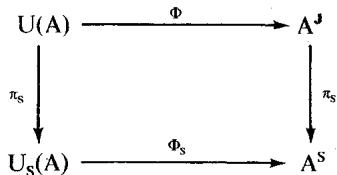
\includegraphics[keepaspectratio]{images/part001_3bc9714d.jpg}}

\(\mathrm{where}\ \Phi_{\mathbf{S}}((a_n)_{n\in \mathbf{S}}) = (\Phi_n((a_d)_{d\in \mathbf{J}_n}))_{n\in \mathbf{S}}.\)

\begin{enumerate}
\def\labelenumi{\alph{enumi})}
\setcounter{enumi}{1}
\item
  For every \(n \in \mathbf{J}\) , \(\operatorname{Ker}(\pi_{\mathrm{S}})\) is stable under \(\mathbf{V}_{n}\) , and \(\operatorname{Ker}(\pi_{\mathrm{S}})\) contains \(\mathbf{V}_{n}(\mathrm{U}(\mathrm{A}))\) if \(n \notin S\) . By passage to the quotient \(\mathbf{V}_{n}\) defines an endomorphism, still denoted \(\mathbf{V}_{n}\) , of the additive group of \(\mathrm{U}_{\mathrm{S}}(\mathrm{A})\) .
\item
  If \(n \in \mathbf{J}\) and if \(n\mathbf{S} \subset \mathbf{S}\) then \(\operatorname{Ker}(\pi_{\mathbf{S}})\) is stable under \(\mathbf{F}_{n}\) , which defines, by passing to the quotient, an endomorphism, still denoted \(\mathbf{F}_{n}\) , of the ring \(\mathrm{U}_{\mathrm{S}}(\mathrm{A})\) .
\end{enumerate}

\(d)\) Let \(n \in \mathbf{J}\) . The ring \(\mathrm{U}_{\mathrm{S}}(\mathrm{A})\) will also be denoted \(\mathrm{U}_{n}(\mathrm{A})\) if \(S = \mathbf{J}_{n}\) , and \(\mathrm{U}_{n\infty}(\mathrm{A})\) if \(\mathrm{S} = \bigcup_{n > 1} \mathbf{J}_{n}\) .

Let \(p\) a prime number. Show that \(\mathrm{U}_{p^{\infty}}(\mathbf{A})\) is identified with the Witt ring \(\mathrm{W}(\mathbf{A})\) and that, for every \(n \in \mathbf{N}\) , \(\mathrm{U}_{p^n}(\mathbf{A})\) is identified with the ring \(\mathrm{W}_{n+1}(\mathbf{A})\) (we identify the element ( \(u_1, u_p, u_{p^2}, ..., u_{p^{n-1}}, u_{p^n}\) ) of \(\mathrm{U}_{p^n}(\mathbf{A})\) to the Witt vector \([a_0, ..., a_n]\) with \(a_i = u_{p^i}\) for \(0 \leqslant i \leqslant n\) ). Group endomorphisms \(\mathbf{V}_p\) and \(\mathbf{F}_p\) of \(\mathrm{U}_{p^\infty}(\mathbf{A})\) correspond respectively, under this identification, to the shift and to the Frobenius endomorphism of \(\mathrm{W}(\mathbf{A})\) .

\begin{enumerate}
\def\labelenumi{\arabic{enumi})}
\setcounter{enumi}{39}
\tightlist
\item
  Let A be a ring. Let \(\mathbf{J} = \mathbf{P} \times \mathbf{Q}\) be a decomposition of the monoid J as a product of submonoids P and Q (which are therefore generated by the prime numbers they contain). One assumes that every \(q \in \mathbf{Q}\) is invertible in A, hence also in U(A) (p.~52, exerc. 35, e)). a) For every \(a \in \mathrm{U(A)}\) the series
\end{enumerate}

\[
\varepsilon_ {\mathbf {Q}} (\boldsymbol {a}) = \sum_ {q \in \mathbf {Q}} \frac {\mu (q)}{q} \mathbf {V} _ {q} \mathbf {F} _ {q} (a),
\]

where \(\mu\) denotes the Möbius function (Lie, II, p.~71), is convergent for the product topology of U(A) = A \(^{J}\) . One thus defines the additive endomorphism \(\varepsilon_{Q} = \sum_{q \in Q} \frac{\mu(q)}{q} V_{q} F_{q}\) of U(A). For every \(n \in J\) , the map \(\Phi_{n} \circ \varepsilon_{Q}\) from U(A) into A is equal to 0 if \(n \notin P\) and to \(\Phi_{n}\) if \(n \in P\) . b) For every \(q \in Q\) , \(q \neq 1\) , one has

\[
\varepsilon_ {\mathbf {Q}} \mathbf {V} _ {q} = 0 = \mathbf {F} _ {q} \varepsilon_ {\mathbf {Q}}.
\]

(Use exerc. 36, c), p.~52.)

\begin{enumerate}
\def\labelenumi{\alph{enumi})}
\setcounter{enumi}{2}
\tightlist
\item
  Show that \(\varepsilon_{\mathbf{Q}}\) is an idempotent whose image is the intersection of the kernels of the \(\mathbf{F}_{q}\) ( \(q \in \mathbf{Q}, q \neq 1\) ).
\end{enumerate}

For \(m \in \mathbf{J}\) and \(a \in \mathbf{A}\) , compute \(\varepsilon_{\mathrm{Q}} \mathrm{V}_{m} \tau(a)\) . Deduce that the kernel of \(\varepsilon_{\mathrm{Q}}\) is the set of elements of the form \(\sum_{n \in \mathrm{Q}} \mathrm{V}_{n} \tau(a_{n})\) , with \(a_{n} \in \mathbf{A}\) . The subset \(\varepsilon_{\mathrm{Q}} \mathrm{U}(\mathrm{A})\) of \(\mathrm{U}(\mathrm{A})\) is stable under addition and multiplication. Equipped with these two operations, it is a commutative ring, with identity \(\varepsilon_{\mathrm{Q}}(1_{\mathrm{U}(\mathrm{A})})\) and the map \(\varepsilon_{\mathrm{Q}}: \mathrm{U}(\mathrm{A}) \to \varepsilon_{\mathrm{Q}} \mathrm{U}(\mathrm{A})\) is a ring homomorphism.

\begin{enumerate}
\def\labelenumi{\alph{enumi})}
\setcounter{enumi}{3}
\tightlist
\item
  For every \(q \in Q\) , set \(e_{q} = \frac{1}{q} V_{q} \varepsilon_{Q} F_{q}\) . Show that we have \(e_{q}^{2} = e_{q}\) and \(e_{q} e_{q'} = 0\) if \(q \neq q'\) and that, for every \(a \in U(A)\) we have
\end{enumerate}

\[
(*) \quad \boldsymbol {a} = \sum_ {q \in Q} e _ {q} (\boldsymbol {a}),
\]

where the sum is convergent for the product topology of U(A). (For (*) reduce to the case where \(a = X \in \mathrm{U}(\mathbf{R}[\mathbf{X}])\) , R being the subring of Q formed by the rational numbers with denominator in Q. It then suffices to apply \(\Phi\) and to verify the analogue of (*) in \(\mathbf{R}[\mathbf{X}]^{\mathbf{J}}\) which follows from the formula \(\Phi_{pq} \circ e_{q'} = \Phi_{pq} \delta_{qq'}\) if \(p \in P\) , \(q \in Q\) , \(q' \in Q\) .

The subset \(e_q \mathrm{U(A)}\) of \(\mathrm{U(A)}\) is stable under addition and multiplication. Equipped with these two operations, it is a commutative ring, with identity \(e_q(1_{\mathrm{U(A)}})\) and the map \(e_q: \mathrm{U(A)} \to e_q \mathrm{U(A)}\) is a ring homomorphism.

\begin{enumerate}
\def\labelenumi{\alph{enumi})}
\setcounter{enumi}{4}
\tightlist
\item
  For every \(q \in \mathbf{Q}\) , one has \(\mathbf{F}_q e_q = \varepsilon_{\mathbf{Q}} \mathbf{F}_q\) and \(\left(\frac{1}{q} \mathbf{V}_q\right) \varepsilon_{\mathbf{Q}} = e_q \left(\frac{1}{q} \mathbf{V}_q\right)\) . Conclude from this that \(\boldsymbol{a} \mapsto \mathbf{F}_q(\boldsymbol{a})\)
\end{enumerate}

is a ring isomorphism \(e_q\mathrm{U(A)}\to \varepsilon_{\mathrm{Q}}\mathrm{U(A)}\) , with inverse \(\pmb {a}\mapsto \frac{1}{q}\mathbf{V}_q(\pmb {a})\)

\begin{enumerate}
\def\labelenumi{\alph{enumi})}
\setcounter{enumi}{5}
\item
  Show that the canonical projection \(\pi_{\mathbb{P}}: \mathrm{U}(\mathrm{A}) \to \mathrm{U}_{\mathbb{P}}(\mathrm{A})\) (exerc. 39) defines a ring isomorphism \(\varepsilon_{\mathbb{Q}} \mathrm{U}(\mathrm{A}) \to \mathrm{U}_{\mathbb{P}}(\mathrm{A})\) . Deduce a ring isomorphism from U(A) onto \(\mathrm{U}_{\mathbb{P}}(\mathrm{A})^{\mathbb{Q}}\) sending \(a\) to \((\pi_{\mathbb{P}} \varepsilon_{\mathbb{Q}} \mathrm{F}_{q}(a))_{q \in \mathbb{Q}}\) for every \(a \in \mathrm{U}(\mathrm{A})\) .
\item
  If A is a Q-algebra, one may take \(\mathbf{P} = \{1\}\) and \(\mathbf{Q} = \mathbf{J}\) . One deduces a ring isomorphism \(\mathrm{U}(\mathrm{A}) \to \mathrm{A}^{\mathbf{J}}\) , which is none other than \(\Phi\) .
\end{enumerate}

  \(h)\) Suppose that \(\mathbf{P} = \{p^n | n \in \mathbb{N}\}\) , where \(p\) is a prime number. Thus every prime number \(q \neq p\) is invertible in A. We obtain a ring isomorphism \(\mathrm{U(A)} \to \mathrm{W(A)}^{\mathrm{Q}}\) (cf.~exerc. 39, \(d\) )).

We shall denote \(\omega_{\mathrm{A}}\) the map from W(A) to U(A), which, via the isomorphism between U(A) and \(\mathrm{W(A)}^{\mathbf{Q}}\), corresponds to the inclusion of W(A) in \(\mathrm{W(A)}^{\mathbf{Q}}\) according to the first component.

\begin{enumerate}
\def\labelenumi{\arabic{enumi})}
\setcounter{enumi}{40}
\tightlist
\item
  Let A be a ring.
\end{enumerate}

\begin{enumerate}
\def\labelenumi{\alph{enumi})}
\tightlist
\item
  Let \(\mu: A \to U(A)\) a ring homomorphism such that \(\Phi_1 \circ \mu = \text{Id}_A\) . Put \(\sigma = \Phi \circ \mu\) and \(\sigma(a) = (\sigma_n(a))_{n \in J}\) for \(a \in A\) . The maps \(\sigma_n: A \to A (n \in J)\) satisfy the following conditions:
\end{enumerate}

\begin{enumerate}
\def\labelenumi{(\arabic{enumi})}
\item
  \(\sigma_{n}\) is a ring homomorphism for all \(n\in\mathbf{J}\) , and \(\sigma_{1}=\mathrm{Id}_{\mathbf{A}}\) .
\item
  For every prime number \(p\) and for all \(a \in \mathbf{A}\) , one has \(\sigma_p(a) \equiv a^p \mod p\mathbf{A}\) and
\end{enumerate}

\[
\sigma_ {p} \left(\sigma_ {n} (a)\right) \equiv \sigma_ {p n} (a) \bmod . p ^ {w _ {p} (p n)} \mathrm{A} \quad \text { for every } \quad n \in \mathbf {J}.
\]

\begin{enumerate}
\def\labelenumi{\alph{enumi})}
\setcounter{enumi}{1}
\item
  Suppose that the additive group of A is Z-torsion-free. Let \(\sigma = (\sigma_n)_{n \in \mathbf{J}}\) be a family of mappings \(\sigma_n: A \to A\) satisfying conditions (1) and (2) of \(a\) ). There exists a unique ring homomorphism \(\mu: A \to U(A)\) such that \(\Phi_1 \circ \mu = Id_A\) and \(\Phi \circ \mu = \sigma\) (Apply Exercises 32 and 33, \(d\) ), p.~51.)
\item
  Suppose that the additive group of A is Z-torsion-free. There exists a unique ring homomorphism
\end{enumerate}

\[
\mu^ {\mathrm{A}}: \mathrm{U} (\mathrm{A}) \rightarrow \mathrm{U} (\mathrm{U} (\mathrm{A}))
\]

such that \(\Phi^{\mathrm{U(A)}}\circ \mu^{\mathrm{A}}\) is the map

\[
\mathbf {F} ^ {\mathbf {A}}: \mathrm{U} (\mathbf {A}) \rightarrow \mathrm{U} (\mathbf {A}) ^ {\mathbf {J}}
\]

defined by \(\mathbf{F}^{\mathrm{A}}(\boldsymbol{a}) = (\mathbf{F}_n(\boldsymbol{a}))_{n\in \mathbf{J}}\) (Reduce to the case where \(\mathbf{A} = \mathbf{Z}[\mathbf{X}]\) . Apply \(b\) ) and Exercises 36 and 38, \(b\) ), pp. 52 and 53.)

\begin{enumerate}
\def\labelenumi{\alph{enumi})}
\setcounter{enumi}{3}
\tightlist
\item
  Let \(\mathbf{X} = (\mathbf{X}_n)_{n\in \mathbf{J}}\) be a family of indeterminates considered as an element of \(\mathrm{U}(\mathbf{Z}[\mathbf{X}])\). Let
\end{enumerate}

\[
\mu^ {\mathbf {Z} [ \mathbf {X} ]} (\mathbf {X}) = \left(\mu_ {n} (\mathbf {X})\right) _ {n \in \mathbf {J}} = \left(\left(\mu_ {n, m} (\mathbf {X})\right) _ {m \in \mathbf {J}}\right) _ {n \in \mathbf {J}}
\]

where \(\mu_{n,m}(\mathbf{X})\in\mathbf{Z}[\mathbf{X}]\) for \(n,m\in\mathbf{J}\). For every ring A define \(\mu^{\mathbf{A}}:\mathrm{U}(\mathbf{A})\to\mathrm{U}(\mathrm{U}(\mathbf{A}))\) by \(\mu^{\mathbf{A}}(\boldsymbol{a})=(\left(\mu_{n,m}(\boldsymbol{a})\right)_{m\in\mathbf{J}})_{n\in\mathbf{J}}\). Show that \(\mu^{\mathbf{A}}\) is a ring homomorphism such that the following diagram is commutative

\begin{enumerate}
\def\labelenumi{(\arabic{enumi})}
\tightlist
\item
\end{enumerate}

\pandocbounded{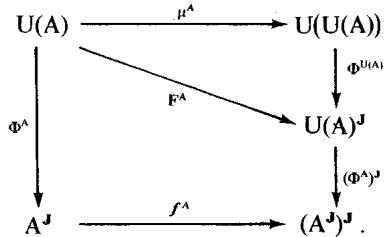
\includegraphics[keepaspectratio]{images/part001_e852df9c.jpg}}

Here by definition, \(f^{\mathrm{A}}(\boldsymbol{a}) = (f_n(\boldsymbol{a}))_{n \in \mathbf{J}}\) for \(\boldsymbol{a} \in \mathrm{A}^{\mathrm{J}}\) , and \(\Phi^{\mathrm{A}}\) (resp. \(\Phi^{\mathrm{U(A)}}\) ) is the homomorphism \(\Phi\) associated with the ring A (resp. U(A)).

\begin{enumerate}
\def\labelenumi{\alph{enumi})}
\setcounter{enumi}{4}
\tightlist
\item
  For every ring homomorphism \(\rho: \mathbf{B} \to \mathbf{A}\) the diagram
\end{enumerate}

\pandocbounded{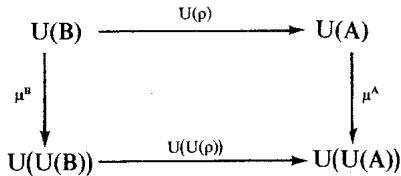
\includegraphics[keepaspectratio]{images/part001_6be88655.jpg}}

is commutative.

\begin{enumerate}
\def\labelenumi{\alph{enumi})}
\setcounter{enumi}{5}
\tightlist
\item
  Show that the following diagram is commutative.
\end{enumerate}

\pandocbounded{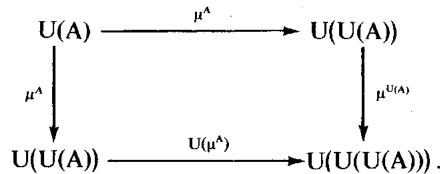
\includegraphics[keepaspectratio]{images/part001_4b4fe1b3.jpg}}

(Reduce to the case where A = \(\mathbf{Q}[\mathbf{X}]\). Then A is a Q-algebra, hence \(\Phi^{\mathbf{A}}: \mathrm{U}(\mathrm{A}) \to \mathrm{A}^{\mathbf{J}}\) is an isomorphism and U(A) is also a Q-algebra. If, using diagram (1) and by transport of structure, one replaces \(\mu^{\mathbf{A}}\) by \(f^{\mathbf{A}}\) when A is a Q-algebra, one is reduced to proving the commutativity of the diagram

\pandocbounded{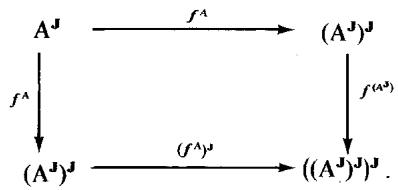
\includegraphics[keepaspectratio]{images/part001_85799ba9.jpg}}

We have

\[
f ^ {(\mathrm{A} ^ {\mathrm{J}})} \left(f ^ {\mathrm{A}} (\mathbf {X})\right) = f ^ {(\mathrm{A} ^ {\mathrm{J}})} \left(\left(f _ {n} (\mathbf {X})\right) _ {n \in \mathbf {J}}\right) = \left(\left(f _ {m} \left(f _ {n} (\mathbf {X})\right)\right) _ {n \in \mathbf {J}}\right) _ {m \in \mathbf {J}} = \left(\left(f _ {m n} (\mathbf {X})\right) _ {n \in \mathbf {J}}\right) _ {m \in \mathbf {J}},
\]

and

\[
(f ^ {\mathrm{A}}) ^ {\mathrm{J}} (f ^ {\mathrm{A}} (\mathbf {X})) = (f ^ {\mathrm{A}}) ^ {\mathrm{J}} ((f _ {n} (\mathbf {X})) _ {n \in \mathbf {J}}) = (f ^ {\mathrm{A}} (f _ {n} (\mathbf {X}))) _ {n \in \mathbf {J}} = ((f _ {m n} (\mathbf {X})) _ {m \in \mathbf {J}}) _ {n \in \mathbf {J}}.
\]

\begin{enumerate}
\def\labelenumi{\alph{enumi})}
\setcounter{enumi}{6}
\tightlist
\item
  For every \(a \in \mathbf{A}\) , one has
\end{enumerate}

\[
\mu_ {n} ^ {\mathrm{A}} (\tau (a)) = 0 \quad \text { for } \quad n \geqslant 2.
\]

\begin{enumerate}
\def\labelenumi{\alph{enumi})}
\setcounter{enumi}{7}
\tightlist
\item
  We have the following commutative diagram
\end{enumerate}

\pandocbounded{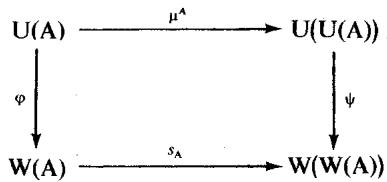
\includegraphics[keepaspectratio]{images/part001_0d6c50d0.jpg}}

where the map \(s_{\mathbf{A}}\) is the one defined in exerc. 15, p.~44, where the map \(\varphi\) from U(A) to W(A) is obtained by identifying W(A) with U \(_{p\infty}\) (A) (p.~53, exerc. 39), and the map \(\psi\) is the composite of U( \(\varphi\) ) and the map from U(W(A)) to W(W(A)) obtained by identifying W(W(A)) with U \(_{p\infty}\) (W(A)).

\begin{enumerate}
\def\labelenumi{\arabic{enumi})}
\setcounter{enumi}{41}
\tightlist
\item
  Let A be a ring and T an indeterminate. We denote by \(\Lambda(A)\) (or \(\Lambda_{T}(A)\) ) the set \(1 + TA[[T]]\) of formal power series with coefficients in A and constant term equal to 1; it is a subgroup of the multiplicative group of \(A[[T]]\). We define
\end{enumerate}

\[
\mathrm{L}: \Lambda (\mathrm{A}) \rightarrow \mathrm{A} ^ {\mathbf {J}}, \quad \mathrm{L} (f) = \left(\mathrm{L} _ {n} (f)\right) _ {n \in \mathbf {J}},
\]

by

\[
- \mathrm{T} \frac {d f}{d \mathrm{T}} / f = \sum_ {n \in \mathbf {J}} \mathrm{L} _ {n} (f) (- \mathrm{T}) ^ {n}.
\]

\begin{enumerate}
\def\labelenumi{\alph{enumi})}
\item
  Show that one has L(fg) = L(f) + L(g) for any f, g ∈ Λ(A).
\item
  If A is a Q-algebra, then L is bijective, its inverse ε being given by
\end{enumerate}

\[
\varepsilon (\boldsymbol {a}) = \exp (- \sum_ {n \in \mathbf {J}} \frac {a _ {n}}{n} (- \mathrm{T}) ^ {n})
\]

for \(a \in A^{J}\) .

\begin{enumerate}
\def\labelenumi{\arabic{enumi})}
\setcounter{enumi}{42}
\tightlist
\item
  Let E: U(A) → Λ(A) be the map defined by
\end{enumerate}

\[
\mathrm{E} (\boldsymbol {a}) = \prod_ {n \in \mathbf {J}} (1 - a _ {n} (- \mathrm{T}) ^ {n})
\]

for \(a \in \mathrm{U}(\mathrm{A})\) .

\begin{enumerate}
\def\labelenumi{\alph{enumi})}
\tightlist
\item
  Prove the commutativity of the diagram.
\end{enumerate}

\pandocbounded{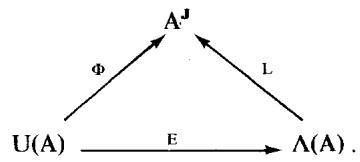
\includegraphics[keepaspectratio]{images/part001_4add4456.jpg}}

Deduce that if A is a Q-algebra, then

\[
\prod_ {n \in \mathbf {J}} (1 - a _ {n} \mathrm{T} ^ {n}) = \exp \left(- \sum_ {n \in \mathbf {J}} (\Phi_ {n} (\boldsymbol {a}) / n) \mathrm{T} ^ {n}\right)
\]

for all \(a \in \mathrm{U}(\mathrm{A})\) .

\begin{enumerate}
\def\labelenumi{\alph{enumi})}
\setcounter{enumi}{1}
\item
  Show that E is bijective. (If one sets \(\prod_{n\in J}(1 - a_n(-T)^n) = \sum_{n\geqslant 0}c_n(a)(-T)^n\) it suffices to apply exerc. 33, a), p.~51 to the family of polynomials \(c_{n}(\mathbf{X})\) of \(\mathbf{Z}[\mathbf{X}]\) .)
\item
  We equip \(\Lambda(A)\) with the unique ring structure such that E is a ring isomorphism. Show that the addition of \(\Lambda(A)\) is the multiplication of series, with identity element 1. The multiplication of the ring \(\Lambda(A)\) denoted \((f,g)\mapsto f*g\) , is defined by the formula
\end{enumerate}

\[
\mathrm{E} (\boldsymbol {a} \times \boldsymbol {b}) = \mathrm{E} (\boldsymbol {a}) * \mathrm{E} (\boldsymbol {b})
\]

for any \(a, b \in \mathrm{U}(\mathrm{A})\) ; its identity element is \(1 + T\) .

\begin{enumerate}
\def\labelenumi{\alph{enumi})}
\setcounter{enumi}{3}
\tightlist
\item
  Let \(\tau : \mathrm{A} \to \mathrm{U}(\mathrm{A})\) be the map defined in exerc. 37, c), p.~53. We have
\end{enumerate}

\[
\begin{array}{c} \mathrm{E} (\tau (a)) = 1 + a \mathrm{T} \\ (1 + a \mathrm{T}) * (1 + b \mathrm{T}) = 1 + a b \mathrm{T} \\ (1 + a \mathrm{T}) * f (\mathrm{T}) = f (a \mathrm{T}) \\ \mathrm{L} (1 + a \mathrm{T}) = (a ^ {n}) _ {n \in \mathbf {J}} \end{array}
\]

for any \(a, b\) in \(\mathbf{A}\) and \(f(\mathbf{T})\) in \(\Lambda(\mathbf{A})\) .

\begin{enumerate}
\def\labelenumi{\alph{enumi})}
\setcounter{enumi}{4}
\tightlist
\item
  Let \(f\) and \(g\) two elements of \(\Lambda(A)\) that are polynomials in \(T\) , and let \(m\) the degree of \(f\) . Put
\end{enumerate}

\[
\varphi (\mathrm{X}) = \mathrm{X} ^ {m} f (\mathrm{T} / \mathrm{X})
\]

and

\[
\gamma (\mathrm{X}) = g (- \mathrm{X}).
\]

These are polynomials in X with coefficients in A\([\mathrm{T}]\); \(\varphi\) is monic and \(f*g\) is the resultant \(\operatorname{res}(\varphi, \gamma)\) of the polynomials \(\varphi\) and \(\gamma\) (cf. A, IV, p. 75).

(One may start from the formula

\[
(1 + a \mathrm{T}) * g = g (a \mathrm{T}),
\]

deduce the result if \(A = \mathbf{Z}[X_{1}, \ldots, X_{m}]\) and \(f = \prod_{i=1}^{m} (1 + X_i \mathrm{T})\), and pass from there to the general case.)

\begin{enumerate}
\def\labelenumi{\arabic{enumi})}
\setcounter{enumi}{43}
\tightlist
\item
  Let A be a ring.
\end{enumerate}

\begin{enumerate}
\def\labelenumi{\alph{enumi})}
\item
  The set \(\hat{\mathbf{U}}(\mathbf{A})\) of elements of \(\mathrm{U}(\mathbf{A})\) with nilpotent coordinates, all but finitely many of which are zero, is an ideal of the ring \(\mathrm{U}(\mathbf{A})\) . For every \(n \in \mathbf{J}\) , it is stable under \(\mathrm{F}_n\) and \(\mathrm{V}_n\) .
\item
  Let \(\boldsymbol{a} \in \hat{\mathbf{U}}(\mathbf{A})\) . Then the element \(\mathrm{E}(\boldsymbol{a})\) of \(\Lambda(\mathbf{A})\) is a polynomial in T. Its value at \(-1\) is an invertible element of A, which is also, for every \(n \in \mathbf{J}\) , the value at \(-1\) of the polynomial \(\mathrm{E}(\mathrm{V}_n\boldsymbol{a})\) .
\item
  If \(\boldsymbol{a} \in \mathrm{U}(\mathbf{A})\) and \(\boldsymbol{b} \in \hat{\mathbf{U}}(\mathbf{A})\) , denote by \(\langle \boldsymbol{a}, \boldsymbol{b} \rangle\) the value at \(-1\) of the polynomial \(\mathrm{E}(\boldsymbol{a}\boldsymbol{b})\) . One thus defines a Z-bilinear map from \(\mathrm{U}(\mathbf{A}) \times \hat{\mathbf{U}}(\mathbf{A})\) into \(\mathbf{A}^*\) and one has
\end{enumerate}

\[
\begin{array}{l} \langle \mathbf {F} _ {n} \boldsymbol {a}, \boldsymbol {b} \rangle = \langle \boldsymbol {a}, \mathbf {V} _ {n} \boldsymbol {b} \rangle \\ \langle \mathbf {V} _ {n} \boldsymbol {a}, \boldsymbol {b} \rangle = \langle \boldsymbol {a}, \mathbf {F} _ {n} \boldsymbol {b} \rangle \quad \text { for every } n \in \mathbf {J}. \end{array}
\]

\begin{enumerate}
\def\labelenumi{\arabic{enumi})}
\setcounter{enumi}{44}
\tightlist
\item
  By pre-λ-ring one means a ring A equipped with maps \(\lambda_{n}: \mathbf{A} \to \mathbf{A} (n \in \mathbb{N})\) such that (i) \(\lambda_{0}(a) = 1\) ,
\end{enumerate}

\begin{enumerate}
\def\labelenumi{(\roman{enumi})}
\setcounter{enumi}{1}
\item
  \(\lambda_{1}(a) = a,\)
\item
  \(\lambda_{n}(a + b) = \sum_{p=0}^{n} \lambda_{p}(a) \lambda_{n-p}(b)\) ,
\end{enumerate}

for any \(a, b\) in A. Conditions (i) and (iii) are also expressed by saying that

\[
\lambda (a) = \sum_ {n \geqslant 0} \lambda_ {n} (a) \mathrm{T} ^ {n}
\]

defines a homomorphism from the additive group of A into the multiplicative group \(\Lambda(A)\) .

By \(\lambda\) -morphism of a pre- \(\lambda\) -ring A into another B, one means a homomorphism \(\rho: A \to B\) of rings such that \(\rho(\lambda_n(a)) = \lambda_n(\rho(a))\) for any \(a \in A\) , \(n \in \mathbf{N}\) , in other words such that the diagram

\pandocbounded{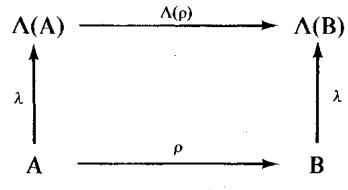
\includegraphics[keepaspectratio]{images/part001_12576e27.jpg}}

is commutative (the map \(\Lambda(\rho)\) transforms the series \(1 + \sum_{n\geqslant 1}a_n\mathrm{T}^n\) into the series \(1 + \sum_{n\geqslant 1}\rho(a_n)\mathrm{T}^n\) ). Let A be a ring. We propose to equip \(\Lambda(\mathbf{A})\) with a pre- \(\lambda\) -ring. Let us denote \(\mathbf{E}^{\mathbf{A}}:\mathrm{U}(\mathbf{A})\to \Lambda_{\mathbf{T}}(\mathbf{A})\) the ring isomorphism defined in exerc. 43. Let S be another indeterminate.

\begin{enumerate}
\def\labelenumi{\alph{enumi})}
\tightlist
\item
  Show that the two composed isomorphisms
\end{enumerate}

\[
\mathrm{U} (\mathrm{U} (\mathrm{A})) \xrightarrow {\mathrm{U} (\mathrm{E} ^ {\mathrm{A}})} \mathrm{U} (\Lambda_ {\mathrm{T}} (\mathrm{A})) \xrightarrow {\mathrm{E} ^ {\Lambda_ {\mathrm{T}} (\mathrm{A})}} \Lambda_ {\mathrm{S}} (\Lambda_ {\mathrm{T}} (\mathrm{A}))
\]

and

\[
\mathrm{U} (\mathrm{U} (\mathrm{A})) \xrightarrow {\mathrm{E} ^ {\mathrm{U} (\mathrm{A})}} \Lambda_ {\mathrm{S}} (\mathrm{U} (\mathrm{A})) \xrightarrow {\Lambda_ {\mathrm{S}} (\mathrm{E} ^ {\mathrm{A}})} \Lambda_ {\mathrm{S}} (\Lambda_ {\mathrm{T}} (\mathrm{A}))
\]

coincide; we will denote them \(\tilde{\mathbf{E}}^{\mathbf{A}}\) .

We define the map \(\lambda^{\mathrm{A}}\) by the commutativity of the diagram

\pandocbounded{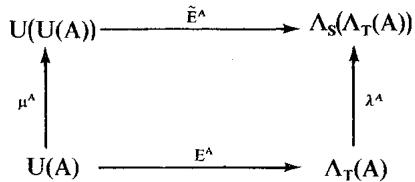
\includegraphics[keepaspectratio]{images/part001_a93606d8.jpg}}

where \(\mu^{\mathbf{A}}\) denotes the homomorphism defined in exerc. 41, \(d\) ), p.~55.

\begin{enumerate}
\def\labelenumi{\alph{enumi})}
\setcounter{enumi}{1}
\item
  The ring \(\Lambda(A)\), equipped with \(\lambda^{A}\), is a pre-\(\lambda\)-ring. For every ring homomorphism \(\rho: A \to B\), \(\Lambda(\rho): \Lambda(A) \to \Lambda(B)\) is a \(\lambda\)-morphism.
\item
  A pre-λ-ring A is called a λ-ring if λ: A → Λ(A) is a λ-morphism (for the pre-λ-ring structure on Λ(A) just defined).
\end{enumerate}

Let A be a ring. Show that \((\Lambda(A), \lambda^A)\) is a \(\lambda\)-ring. (Use Exerc. 41, \(f\) ), p.~56.)

\begin{enumerate}
\def\labelenumi{\arabic{enumi})}
\setcounter{enumi}{45}
\tightlist
\item
  \begin{enumerate}
  \def\labelenumii{\alph{enumii})}
  \tightlist
  \item
    Let A be a pre-λ-ring and \(a \in A\) . The λ-rank of a is called the least upper bound in \(\overline{R}\) of the set of integers \(n \in N\) such that \(\lambda_{n}(a) \neq 0\) . Let P be a multiplicative subset of A consisting of elements of λ-rank \(\leqslant 1\) . Let \(a = \sum_{i \in I} a_{i}\) be the sum of a finite family of elements of P. We have \(\lambda(a) = \prod_{i \in I} (1 + a_i T)\) , hence \(\lambda_n(a) = s_n((a_i)_{i \in I})\) , where \(s_n\) denotes the elementary symmetric polynomial
  \end{enumerate}
\end{enumerate}

of degree n (A, IV, p.~63).

\begin{enumerate}
\def\labelenumi{\alph{enumi})}
\setcounter{enumi}{1}
\item
  Let A be a ring and \(a, b\) elements of A. Then in \(\Lambda(A)\) the elements \(1 + aT\) and \((1 + aT)*(1 + bT) = 1 + abT\) are of \(\lambda\) -rank \(\leqslant 1\) .
\item
  Let A be a pre-λ-ring. Suppose there exists a multiplicative submonoid of A, consisting of elements of λ-rank ≤ 1, which generates the additive group of A. Show that A is then a λ-ring. More generally, A is a λ-ring if there exists an injective λ-morphism from A into a pre-λ-ring satisfying the preceding property ("Splitting principle"). (It is a matter of showing that the Z-bilinear map \((a, b) \mapsto \lambda(a) * \lambda(b) * \lambda(ab)^{-1}\) is zero and that the Z-linear maps \(a \mapsto \Lambda_{\mathrm{S}}(\lambda_{\mathrm{T}})[\lambda_{\mathrm{S}}(a)]\) and \(a \mapsto \lambda_{\mathrm{S}}^{\mathrm{A}}(\lambda_{\mathrm{T}}(a))\) from A to \(\Lambda_{\mathrm{S}}(\Lambda_{\mathrm{T}}(\mathrm{A}))\) coincide. It suffices to verify these properties for \(a, b \in P\) .)
\item
  Let \(A = \mathbf{Z}[(X_i)_{i\in I}, (X_{i'}')_{i'\in I'}]\) be the ring of polynomials in two finite families of indeterminates. We have
\end{enumerate}

\[
\prod_ {i \in I} (1 + X _ {i} T) = \sum_ {n \geqslant 0} s _ {n} ((X _ {i}) _ {i \in I}) T ^ {n}
\]

where

\[
s _ {n} \left(\left(X _ {i}\right) _ {i \in I}\right) = \sum_ {\mathrm{H} \in \binom {I} {n}} X _ {\mathrm{H}},
\]

\(\binom{I}{n}\) denoting the set of subsets with n elements of I, and where \(X_{H} = \prod_{h \in H} X_{h}\) . By assigning to the \(X_{i}\) (and \(X_{i'}\) ) the weight 1, \(s_{n}\) is homogeneous of weight n. Every symmetric polynomial in \((X_{i})_{i \in I}\) is expressed uniquely as a polynomial in the \(s_{n}\) ( \(n \geqslant 1\) ) (A, IV, p.~58). In particular, for every \(m \geqslant 0\) , one has

\[
s _ {m} \left(\left(\mathrm{X} _ {\mathrm{H}}\right) _ {\mathrm{H} \in \binom {\mathrm{I}} {n}}\right) = \mathrm{Q} _ {n, m} \left(s _ {1}, \dots , s _ {n m}\right)
\]

where \(Q_{n,m}\) is homogeneous of weight nm in the \(s_r = s_r((X_i)_{i \in I}) (r = 1, \ldots, nm)\) . This is the coefficient of \(T^m\) in \(\prod (1 + X_H T)\) , and it is well defined and independent of I, provided that \(\text{Card}(I) \geqslant nm\) .

The coefficient of \(\mathbf{T}^n\) in \(\prod (1 + X_iX_i'T)\) is

\[
s _ {n} \left(\left(X _ {i} X _ {i ^ {\prime}} ^ {\prime}\right) _ {(i, i ^ {\prime}) \in I \times I ^ {\prime}}\right) = P _ {n} \left(s _ {1}, \dots , s _ {n}, s _ {1} ^ {\prime}, \dots , s _ {n} ^ {\prime}\right)
\]

where \(s_r' = s_r((X_{i'}')_{i'\in I'})\) , and where \(P_n\) is homogeneous of weight \(n\) in each of the families of variables \((s_r)\) and \((s_r')\) . It is well defined and independent of I and I' provided that I and I' have cardinalities \(\geqslant n\) .

Show that in the \(\lambda\) -ring \(\Lambda(A)\) we have

\[
\left(\sum_ {r \geqslant 0} s _ {r} \mathrm{T} ^ {r}\right) * \left(\sum_ {r \geqslant 0} s _ {r} ^ {\prime} \mathrm{T} ^ {r}\right) = \sum_ {n \geqslant 0} \mathrm{P} _ {n} (s _ {1},..., s _ {n}, s _ {1} ^ {\prime},..., s _ {n} ^ {\prime}) \mathrm{T} ^ {n}
\]

and

\[
\lambda_ {n} ^ {\mathrm{A}} \left(\sum_ {r \geqslant 0} s _ {r} \mathrm{T} ^ {r}\right) = \sum_ {m \geqslant 0} \mathrm{Q} _ {n, m} \left(s _ {1}, \dots , s _ {n m}\right) \mathrm{T} ^ {m}.
\]

By a) and b), we have

\[
\left(\sum_ {r} s _ {r} \mathrm{T} ^ {r}\right) * \left(\sum_ {r} s _ {r} ^ {\prime} \mathrm{T} ^ {r}\right) = \left(\prod_ {i} \left(1 + \mathrm{X} _ {i} \mathrm{T}\right)\right) * \left(\prod_ {i ^ {\prime}} \left(1 + \mathrm{X} _ {i} ^ {\prime} \mathrm{T}\right)\right) = \prod_ {i, i ^ {\prime}} \left(1 + \mathrm{X} _ {i} \mathrm{X} _ {i ^ {\prime}} ^ {\prime} \mathrm{T}\right)
\]

and

\[
\begin{array}{l} \lambda (\sum_ {r} s _ {r} \mathrm{T} ^ {r}) = \lambda (\prod _{i} (1 + X _ {i} \mathrm{T})) = \prod _{i} (1 + (1 + X _ {i} \mathrm{T}) \mathrm{S}) = \sum _{n} s _ {n} ((1 + X _ {i} \mathrm{T}) _ {i \in \mathrm{I}}) \mathrm{S} ^ {n} \\ \text{and}\quad s _ {n} ((1 + X _ {i} \mathrm{T}) _ {i \in \mathrm{I}}) = \prod _{\mathrm{H} \in \binom {\mathrm{I}} {n}} (1 + X _{\mathrm{H}} \mathrm{T}) . \end{array}
\]

\begin{enumerate}
\def\labelenumi{\alph{enumi})}
\setcounter{enumi}{4}
\tightlist
\item
  Let A be a pre-λ-ring. For A to be a λ-ring, it is necessary and sufficient that the following conditions be satisfied, for all a, b in A, and n, m in N.
\end{enumerate}

\begin{enumerate}
\def\labelenumi{(\roman{enumi})}
\item
  \(\lambda(1) = 1 + T,\)
\item
  \(\lambda_{n}(ab) = \mathrm{P}_{n}(\lambda_{1}(a),\dots,\lambda_{n}(a),\lambda_{1}(b),\dots,\lambda_{n}(b)),\)
\item
  \(\lambda_{m}(\lambda_{n}(a)) = Q_{n,m}(\lambda_{1}(a),\dots,\lambda_{nm}(a)).\)
\end{enumerate}

\begin{enumerate}
\def\labelenumi{\alph{enumi})}
\setcounter{enumi}{5}
\tightlist
\item
  Let \(\rho: A \to B\) be a \(\lambda\)-morphism of pre-\(\lambda\)-rings. If A is a \(\lambda\)-ring and \(\rho\) is surjective, then B is a \(\lambda\)-ring. If B is a \(\lambda\)-ring and if \(\rho\) is injective, then A is a \(\lambda\)-ring.
\end{enumerate}

\begin{enumerate}
\def\labelenumi{\arabic{enumi})}
\setcounter{enumi}{46}
\tightlist
\item
  Let A be a ring. We define maps \(F_{n}\) , \(V_{n}\) (\(n \in \mathbf{J}\)) of \(\Lambda(\mathbf{A})\) into itself by the formulas
\end{enumerate}

\[
\mathrm{F} _ {n} (\mathrm{E} (a)) = \mathrm{E} \left(\mathrm{F} _ {n} (a)\right), \quad \mathrm{V} _ {n} (\mathrm{E} (a)) = \mathrm{E} \left(\mathrm{V} _ {n} (a)\right)
\]

for all \(\boldsymbol{a} \in \mathrm{U}(\mathbf{A})\) .

\begin{enumerate}
\def\labelenumi{\alph{enumi})}
\tightlist
\item
  We have \(\mathrm{L}(\mathrm{F}_n(f)) = f_n(\mathrm{L}(f))\) and \(\mathrm{L}(\mathrm{V}_n(f)) = v_n(\mathrm{L}(f))\) for all \(f \in \Lambda(\mathbf{A})\) .
\end{enumerate}

Let n, m be in J and set \(d = \operatorname{pgcd}(n, m)\) .

\begin{enumerate}
\def\labelenumi{\alph{enumi})}
\setcounter{enumi}{1}
\item
  Show that \(F_{n}\) is an endomorphism of the ring \(\Lambda(\mathbf{A})\) , and that we have \(F_{n} \circ F_{m} = F_{nm}\) . For every prime number p and for every \(f \in \Lambda(\mathbf{A})\) , one has \(F_{p}(f) \equiv f^{*p} \mod p * \Lambda(\mathbf{A})\) , where \(f^{*p}\) denotes the product in the ring \(\Lambda(\mathbf{A})\) of p terms equal to f, and where \(p * \Lambda(\mathbf{A})\) denotes the principal ideal of \(\Lambda(\mathbf{A})\) generated by the sum in \(\Lambda(\mathbf{A})\) of p terms equal to the neutral element 1 + T, in other words by \((1 + T)^{p}\) .
\item
  Prove that \(V_{n}\) is an endomorphism of the additive group of \(\Lambda(\mathbf{A})\) , and that we have \(V_{n} \circ V_{m} = V_{nm}\) . d) For every \(f \in \Lambda(\mathbf{A})\) , one has \(F_{n}(V_{m}(f)) = V_{m/d}(F_{n/d}(f))^{d}\) . In particular \(F_{n}(V_{n}(f)) = f^{n}\) , and \(F_{n} \circ V_{m} = V_{m} \circ F_{n}\) if \(d = 1\) . For any \(f,g\in\Lambda(\mathbf{A})\), we have
\item
  For any \(f, g\) in \(\Lambda(A)\) , one has
\end{enumerate}

\[
\begin{array}{l} \mathrm{V} _ {n} (f) * \mathrm{V} _ {m} (g) = \mathrm{V} _ {n m / d} (\mathrm{F} _ {m / d} (f) * \mathrm{F} _ {n / d} (g)) ^ {d}, \\ \mathrm{V} _ {n} (f * \mathrm{F} _ {m} (g)) ^ {n / d} = \mathrm{V} _ {n} (f) * \mathrm{V} _ {n / d} (\mathrm{F} _ {m / d} (g)), \\ \mathrm{V} _ {n} (\mathrm{F} _ {m} (g)) ^ {n / d} = \mathrm{V} _ {n} (1 + \mathrm{T}) * \mathrm{V} _ {n / d} (\mathrm{F} _ {m / d} (g)). \end{array}
\]

In particular, we have

and

\[
\begin{array}{r l} & {\mathrm{V} _ {n} (f) * \mathrm{V} _ {n} (g) = \mathrm{V} _ {n} (f * g) ^ {n}} \\ & {\mathrm{V} _ {n} (f) * \mathrm{V} _ {m} (g) = \mathrm{V} _ {n m} (\mathrm{F} _ {m} (f) * \mathrm{F} _ {n} (g)) \quad \text {if} \quad d = 1.} \end{array}
\]

\begin{enumerate}
\def\labelenumi{\alph{enumi})}
\setcounter{enumi}{5}
\tightlist
\item
  We have
\end{enumerate}

\[
\mathrm{V} _ {n} (f) (\mathrm{T}) = f (- (- \mathrm{T}) ^ {n})
\]

for all \(f \in \Lambda(\mathbf{A})\) . In particular

\[
\mathrm{V} _ {n} (1 + a \mathrm{T}) = 1 - a (- \mathrm{T}) ^ {n}
\]

for every \(a \in \mathbf{A}\) .

\begin{enumerate}
\def\labelenumi{\alph{enumi})}
\setcounter{enumi}{6}
\tightlist
\item
  For every \(a \in \mathbf{A}\) , one has
\end{enumerate}

\[
\mathrm{F} _ {n} (1 + a \mathrm{T}) = 1 + a ^ {n} \mathrm{T}.
\]

For every \(f \in \Lambda(\mathbf{A})\) , one has

\[
\mathrm{F} _ {n} (f) \left(- (- \mathrm{T}) ^ {n}\right) = \mathrm{N} (f (\mathrm{T}))
\]

where N denotes the norm in the extension \(A[[\mathrm{T}^{n}]] \subset A[[\mathrm{T}]]\). (It suffices to treat the case where \(f \in A[\mathrm{T}]\), then embed A into a ring B where f decomposes into a product of linear factors, to which the first formula can be applied.)

For every \(a \in \mathbf{A}\) , one has

\[
\mathrm{F} _ {n} (1 - a (- \mathrm{T}) ^ {m}) = (1 - a ^ {n / d} (- \mathrm{T}) ^ {m / d}) ^ {d}.
\]

(Observe that \(1 - a(-T)^{m} = V_{m}(1 + aT)\) and use c) and f).) h) For any \(a, b \in A\) , one has

\[
(1 - a (- \mathrm{T}) ^ {n}) * (1 - b (- \mathrm{T}) ^ {m}) = (1 - a ^ {m / d} b ^ {n / d} (- \mathrm{T}) ^ {m n / d}) ^ {d}.
\]

(Use the first formula for e).)

\begin{enumerate}
\def\labelenumi{\arabic{enumi})}
\setcounter{enumi}{47}
\tightlist
\item
  Let A be a pre-λ-ring. Denote by Ψ the composite A \(\xrightarrow{\lambda} \Lambda(A) \xrightarrow{L} A^{J}\) , so that \(\Psi(a) = (\psi_{n}(a))_{n \in J}\) , where
\end{enumerate}

\[
- \mathrm{T} \frac {d}{d \mathrm{T}} \lambda (a) / \lambda (a) = \sum_ {n \in \mathrm{J}} \psi_ {n} (a) (- \mathrm{T}) ^ {n}.
\]

More explicitly,

\[
- n \lambda_ {n} (a) = (- 1) ^ {n} \psi_ {n} (a) + (- 1) ^ {n - 1} \psi_ {n - 1} (a). \lambda_ {1} (a) + \dots + (- \psi_ {1} (a)). \lambda_ {n - 1} (a)
\]

for all \(n \in J\) . In particular,

\[
\begin{array}{l} \psi_ {1} (a) = \lambda_ {1} (a) = a \\ \psi_ {2} (a) = \lambda_ {1} (a) ^ {2} - 2 \lambda_ {2} (a) \\ \psi_ {3} (a) = \lambda_ {1} (a) ^ {3} - 3 \lambda_ {1} (a) \lambda_ {2} (a) + 3 \lambda_ {3} (a). \end{array}
\]

The maps \(\psi_{n}:A\to A\) are called Adams operations.

When (A, \(\lambda\) ) = ( \(\Lambda(B)\) , \(\lambda^{B}\) ), where B is a ring, we will also write \(\Psi^{B}\) for \(\Psi\) .

\begin{enumerate}
\def\labelenumi{\alph{enumi})}
\tightlist
\item
  Let B be a ring. Show that for every \(n \in J\) , one has
\end{enumerate}

\[
\psi_ {n} ^ {\mathbf {B}} = \mathrm{F} _ {n}: \Lambda (\mathbf {B}) \rightarrow \Lambda (\mathbf {B}).
\]

(Use the commutative diagram

\pandocbounded{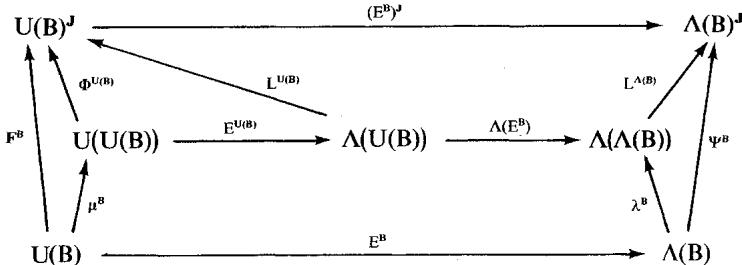
\includegraphics[keepaspectratio]{images/part001_4bd4d5b0.jpg}}

where all the horizontal maps are bijective.)

\begin{enumerate}
\def\labelenumi{\alph{enumi})}
\setcounter{enumi}{1}
\item
  Let A be a pre-λ-ring. For every \(n \in \mathbf{J}\) , \(\psi_n\) is an endomorphism of the additive group of A, and \(\psi_1 = \mathrm{Id}_A\) . If A is a λ-ring, \(\psi_n\) is an endomorphism of the ring A, and \(\psi_n \circ \psi_m = \psi_{nm}\) for any \(n\) , \(m\) in J. Moreover, for every prime number \(p\) we have \(\psi_p(a) \equiv a^p\) mod. \(p\mathbf{A}\) for all \(a \in \mathbf{A}\) (Using the injectivity of \(\lambda: \mathbf{A} \to \Lambda(\mathbf{A})\) and the analogous properties of \(\psi_n^{\mathbf{A}} = \mathbf{F}_n\) .)
\item
  Let A be a pre-λ-ring whose additive group is Z-torsion-free. For A to be a λ-ring, it is necessary and sufficient that the following conditions be satisfied for all integers \(n \geqslant 2\) and \(m \geqslant 2\) :
\end{enumerate}

\begin{enumerate}
\def\labelenumi{(\roman{enumi})}
\item
  \(\psi_n(1) = 1\) ;
\item
  \(\psi_{n}(ab) = \psi_{n}(a)\psi_{n}(b)\) for any \(a,b\) in A;
\item
  \(\psi_{n}\circ \psi_{m} = \psi_{nm}\)
\end{enumerate}

Since L : Λ(A) → A \(^{J}\) is an injective ring homomorphism, Ψ = L ∘ λ is a ring homomorphism if and only if λ is one. Similarly for the diagram.

\pandocbounded{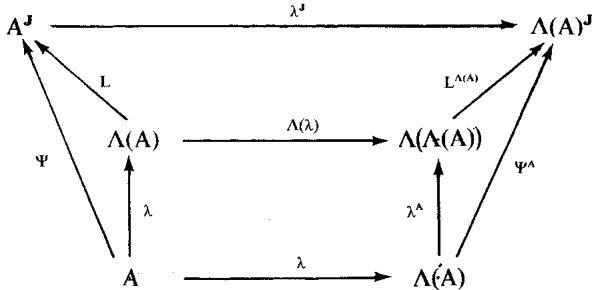
\includegraphics[keepaspectratio]{images/part001_ba507c2f.jpg}}

we deduce that

\(\Lambda (\lambda)\circ \lambda = \lambda^{\mathbf{A}}\circ \lambda\) (λ is a λ-morphism)

\(\Leftrightarrow \lambda^{\mathbf{J}}\circ \Psi = \Psi^{\mathbf{A}}\circ \lambda \Leftrightarrow \lambda \circ \psi_{n} = \psi_{n}^{\mathbf{A}}\circ \lambda\) for every \(n\)

\(\Leftrightarrow \mathrm{L} \circ \lambda \circ \psi_n = \mathrm{L} \circ \psi_n^{\mathrm{A}} \circ \lambda\) for every \(n\) .

Now \(\mathrm{L}\circ \lambda = \Psi\) and \(\mathbf{L}\circ \psi_n^{\mathbf{A}} = \mathbf{L}\circ \mathbf{F}_n = f_n\circ \mathbf{L}.\) Therefore,

\(\Lambda (\lambda)\circ \lambda = \lambda^{\mathrm{A}}\circ \lambda \Leftrightarrow \Psi \circ \psi_{n} = f_{n}\circ \Psi\) for every \(n\)

\(\Leftrightarrow \psi_{m} \circ \psi_{n} = \psi_{nm}\) for any \(m\) and \(n\) .

\begin{enumerate}
\def\labelenumi{\alph{enumi})}
\setcounter{enumi}{3}
\tightlist
\item
  Let A be a λ-ring. Let \(a \in \mathbf{A}\) be an element of λ-rank \(\leqslant 1\) (i.e.\(\lambda(a) = 1 + a\mathbf{T}\) ). Then \(\psi_n(a) = a^n\) for all \(n \in \mathbf{J}\) . If P is a multiplicative subset of A consisting of elements of λ-rank \(\leqslant 1\) and if \(a_1, \ldots, a_r\) belong to P, we have \(\psi_n(a_1 + \cdots + a_r) = a_1^n + \cdots + a_r^n\) .
\end{enumerate}

In the algebra of polynomials \(\mathbf{Z}[(\mathbf{X}_{i})_{i\in I}]\) , denote by \((s_{n})\) the elementary symmetric polynomials, \(\sum_{n\geq0}s_{n}\mathbf{T}^{n}=\prod_{i}(1+\mathbf{X}_{i}\mathbf{T})\) , and

\[
\mathrm{v} _ {n} (s _ {1}, \dots , s _ {n}) = \sum_ {i} \mathrm{X} _ {i} ^ {n}
\]

the n-th Newton polynomial. Show that, for any \(a \in A\) , one has

\[
\psi_ {n} (a) = v _ {n} \left(\lambda_ {1} (a), \dots , \lambda_ {n} (a)\right).
\]

(First verify this relation when \(a\) is of the form \(a_{1} + \cdots + a_{r}\) as above. Passing from there to the case where \(a = 1 + \sum_{h \geqslant 1} s_{h} \mathrm{T}^{h} \in \Lambda(\mathbf{Z}[(\mathrm{X}_{i})_{i \in I}])\) . Next, deduce the general case by embedding A into the \(\lambda\) -ring \(\Lambda(\mathbf{A})\) and using the homomorphism \(\mathbf{Z}[(s_{h})_{h=1,\ldots,n}] \to \mathbf{A}\) which sends \(s_{h}\) onto \(\lambda_{h}(a)\) .)

\begin{enumerate}
\def\labelenumi{\arabic{enumi})}
\setcounter{enumi}{48}
\tightlist
\item
  Let A be a ring, E a finitely generated projective A-module, and \(u \in \text{End}_{\mathbf{A}}(\mathbf{E})\) . If E is a free A-module, we denote by \(\det_{\mathbf{E}}(u)\) the determinant of \(u\) . In general, one can choose an A-module F such that \(\mathbf{E} \oplus \mathbf{F}\) is a finitely generated free A-module, and we set
\end{enumerate}

\[
\det _ {E} (u) = \det _ {E \oplus F} (u \oplus 1 _ {F}).
\]

\begin{enumerate}
\def\labelenumi{\alph{enumi})}
\tightlist
\item
  Show that \(\operatorname{det}_{\mathbf{E}}(u)\) is independent of the choice of F, that \(\operatorname{det}_{\mathbf{E}}(1_{\mathbf{E}}) = 1\) , and that \(\operatorname{det}_{\mathbf{E}}(u \circ v) = \operatorname{det}_{\mathbf{E}}(u) \cdot \operatorname{det}_{\mathbf{E}}(v)\) for any \(u, v\) in \(\operatorname{End}_{\mathbf{A}}(\mathbf{E})\) .
\end{enumerate}
% semantic-fragments: legacy-input-seam
\relax{}
\begin{enumerate}
\def\labelenumi{\alph{enumi})}
\setcounter{enumi}{1}
\tightlist
\item
  Suppose that L is a direct summand submodule of E stable under \(u\), and denote by \(u_{\mathrm{L}} \in \mathrm{End}_{\mathrm{A}}(\mathrm{L})\) and \(u_{\mathrm{E/L}} \in \mathrm{End}_{\mathrm{A}}(\mathrm{E/L})\) the endomorphisms defined by \(u\). Then one has \(\det_{\mathrm{E}}(u) = \det_{\mathrm{L}}(u_{\mathrm{L}}) \cdot \det_{\mathrm{E/L}}(u_{\mathrm{E/L}})\). Let T be an indeterminate, E{[}T{]} = A{[}T{]} \(\otimes_{\mathrm{A}}\) E, and identify \(u\) with \(1_{\mathrm{A[T]}} \otimes_{\mathrm{A}} u \in \mathrm{End}_{\mathrm{A[T]}}(\mathrm{E[T]})\). Put
\end{enumerate}

\[
\chi_ {\mathrm{E}} (u) = \det (\mathrm{T}. 1 - u)
\]

(characteristic polynomial of \(u\)) and

\[
\overline {{{{\chi}}}} _ {\mathrm{E}} (u) = \det (1 + u \mathrm{T}) = \sum_ {n \geqslant 0} \operatorname{Tr} \left(\Lambda ^ {n} (u)\right) \mathrm{T} ^ {n}
\]

where 1 denotes \(1_{\mathrm{E[T]}}\) (cf. A, III, p. 107).

\begin{enumerate}
\def\labelenumi{\alph{enumi})}
\setcounter{enumi}{2}
\item
  We have \(\overline{\chi}_{\mathrm{E}}(0) = 1\). Suppose that E is locally free of constant rank \(r\). We have \(\overline{\chi}_{\mathrm{E}}(1_{\mathrm{E}}) = (1 + \mathrm{T})^{r}\). If \(\sigma_r: \mathrm{A}[\mathrm{T}, \mathrm{T}^{-1}] \to \mathrm{A}[\mathrm{T}, \mathrm{T}^{-1}]\) denotes the mapping \((\sigma_r f)(\mathrm{T}) = \mathrm{T}^r. f((- \mathrm{T})^{-1})\), we have \(\sigma_r(\sigma_r(f)) = (-1)^r f\) and \(\sigma_r(\overline{\chi}_{\mathrm{E}}(u)) = \chi_{\mathrm{E}}(u)\).
\item
  Let \(\alpha: \mathrm{A} \to \mathrm{A}'\) be a ring homomorphism. We have \(\overline{\chi}_{\mathrm{A}'\otimes_{\mathrm{A}}\mathrm{E}}(\mathrm{Id}_{\mathrm{A}'} \otimes_{\mathrm{A}} u) = \alpha(\overline{\chi}_{\mathrm{E}}(u))\), where we denote \(\alpha\) also for the homomorphism \(\mathrm{A}[\mathrm{T}] \to \mathrm{A}'[\mathrm{T}]\) defined by \(\alpha\).
\item
  We have \(\overline{\chi}_{\mathrm{E}}(u) \in \Lambda(\mathrm{A})\) . For every \(n \in \mathbf{J}\) , one has
\end{enumerate}

\[
\begin{array}{l} \lambda_ {n} ^ {\mathrm{A}} (\overline {{\chi}} _ {\mathrm{E}} (u)) = \overline {{\chi}} _ {\Lambda^ {n} (\mathrm{E})} (\Lambda^ {n} (u)), \\ \psi_ {n} ^ {\mathrm{A}} (\overline {{\chi}} _ {\mathrm{E}} (u)) = \overline {{\chi}} _ {\mathrm{E}} (u ^ {n}). \end{array}
\]

(It suffices to verify the formulas locally on the spectrum of A, so we may assume E is equal to \(\mathbf{A}^r\). Let \((u_{ij})_{1\leqslant i,j\leqslant r}\) be the matrix of \(u\), let \((\mathrm{X}_{ij})_{1\leqslant i,j\leqslant r}\) be a family of indeterminates, set \(\mathbf{B} = \mathbf{Z}[(\mathrm{X}_{ij})]\), and let \(v\) be the endomorphism of \(\mathbf{B}^r\) with matrix \(\mathrm{X} = (\mathrm{X}_{ij})_{1\leqslant i,j\leqslant r}\). It suffices to verify the formulas for \(\mathbf{B}^r\) and \(v\in \operatorname {End}_{\mathbf{B}}(\mathbf{B}^r)\). One can embed B in an algebraically closed field C, and it suffices to verify the formulas for \(\mathbf{C}^r\) and \(w = \operatorname {Id}_{\mathbf{C}}\otimes_{\mathbf{B}}v\). Let \(a_1,\dots,a_r\) be the eigenvalues of \(w\), so that \(\overline{\chi}_{\mathbf{C}^r}(w) = \prod_i(1 + a_i\mathrm{T})\). We have \(\psi_n^{\mathrm{C}}(\overline{\chi}_{\mathbf{C}^r}(w)) = \prod_{i = 1}^{r}(1 + a_i^n\mathrm{T}) = \overline{\chi}_{\mathbf{C}^r}(w^n)\). Moreover \(\chi_{\Lambda^n (\mathbf{C}^r)}(\Lambda^n (w)) = \prod_{\mathrm{H}}(1 + a_{\mathrm{H}}\mathrm{T})\), where H ranges over the set of subsets with \(n\) elements of \(\{1,\dots,r\}\), and where \(a_{\mathrm{H}} = \prod_{h\in \mathrm{H}}a_h\). We can now apply Exerc. 46, \(d)\), p.~59, to show that \(\lambda_n^{\mathrm{C}}(\overline{\chi}_{\mathbf{C}^r}(w)) = \overline{\chi}_{\Lambda^{n}(\mathbf{C}^{r})}(\Lambda^{n}(w)).\)

\[
- \mathrm{T} \left[ \frac {d}{d \mathrm{T}} \overline {{{\chi}}} _ {\mathrm{E}} (u) \right] / \overline {{{\chi}}} _ {\mathrm{E}} (u) = \sum_ {n \in \mathbf {J}} \operatorname{Tr} (u ^ {n}) (- \mathrm{T}) ^ {n},
\]

in other words \(\mathrm{L}_n(\overline{\chi}_{\mathrm{E}}(u)) = \mathrm{Tr}(u^n)\) for \(n \in \mathbf{J}\) . (Reason as in \(e\) ).)

\begin{enumerate}
\def\labelenumi{\alph{enumi})}
\setcounter{enumi}{6}
\tightlist
\item
  Let E' be a finitely generated projective A-module, and \(u' \in \mathrm{End}_{\mathbf{A}}(\mathbf{E}')\). In the ring \(\Lambda(\mathbf{A})\),
\end{enumerate}

\[
\overline {{{{\chi}}}} _ {\mathrm{E} \otimes_ {\mathrm{A}} \mathrm{E} ^ {\prime}} (u \otimes_ {\mathrm{A}} u ^ {\prime}) = \overline {{{{\chi}}}} _ {\mathrm{E}} (u) * \overline {{{{\chi}}}} _ {\mathrm{E} ^ {\prime}} (u ^ {\prime}).
\]

(Reason as in e).)

\(h\) ) Let \(k\) be an algebraically closed field of characteristic \(p\ne0\), E a vector space over \(k\) of finite dimension \(n\), and \(u\) an endomorphism of E. We will denote by \(\tilde{\chi}_{\mathrm{E}}(u)\) the image of \(\overline{\chi}_{\mathrm{E}}(u)\) in \(\mathbf{W}(k)\) by the canonical homomorphisms (exerc. 43, p.~57 and exerc. 39, p.~53):

\[
\Lambda (k) \xrightarrow {\mathrm{E} ^ {- 1}} \mathrm{U} (k) \longrightarrow \mathrm{U} _ {p ^ {\infty}} (k) \longrightarrow \mathrm{W} (k).
\]

Prove that if \(\alpha_{1},\ldots,\alpha_{n}\) are the eigenvalues of the endomorphism \(u\) , one has

\[
\tilde {\chi} _ {E} (u) = \sum_ {i = 1} ^ {n} \tau (\alpha_ {i}) \quad \text { in } \quad W (k).
\]

\begin{enumerate}
\def\labelenumi{\arabic{enumi})}
\setcounter{enumi}{49}
\tightlist
\item
  Let A be a pre-λ-ring. By a λ-ideal of A one means an ideal a of A such that λ \(_{n}\) (a) ⊂ a for all n ∈ J.
\end{enumerate}

\begin{enumerate}
\def\labelenumi{\alph{enumi})}
\item
  Let a be a λ-ideal of A. Show that there exists a unique structure λ : A/a → Λ(A/a) of pre-λ-ring on A/a such that the canonical projection A → A/a is a λ-morphism.
\item
  The λ-ideals of A are precisely the kernels of λ-morphisms from A into other pre-λ-rings.
\item
  Let \((\mathfrak{a}_i)_{i\in I}\) be a family of \(\lambda\)-ideals of A. Then \(\bigcap \mathfrak{a}_i\) and \(\sum \mathfrak{a}_i\) are \(\lambda\)-ideals of A.
\item
  Let A be a λ-ring. If α and α′ are λ-ideals of A, then αα′ is a λ-ideal.
\item
  Let A be a \(\lambda\)-ring and let \(a \in \mathbf{A}\). The ideal \(\alpha\) of A generated by \(a, \lambda_2(a), \lambda_3(a), \ldots\) is a \(\lambda\)-ideal.
\end{enumerate}

\begin{enumerate}
\def\labelenumi{\arabic{enumi})}
\setcounter{enumi}{50}
\tightlist
\item
  Let A be a \(\lambda\)-ring and let \((\mathbf{X}_i)_{i\in I}\) be a family of indeterminates. Let us introduce the family of indeterminates \((\lambda_n\mathbf{X}_i)_{(n,i)\in \mathbf{J}\times \mathbf{I}}\) such that \(\lambda_1\mathbf{X}_i = \mathbf{X}_i\) for all \(i\in I\). Consider the polynomial algebra \(\mathrm{B} = \mathrm{A}\big[(\lambda_n\mathbf{X}_i)_{(n,i)\in \mathbf{J}\times \mathbf{I}}\big]\).
\end{enumerate}

The ring homomorphism \(\lambda: A \to \Lambda(A) \subset \Lambda(B)\) extends uniquely to a ring homomorphism \(\lambda: B \to \Lambda(B)\) such that

\[
\lambda (X _ {i}) = 1 + \sum_ {n \in \mathbf {J}} (\lambda_ {n} X _ {i}) T ^ {n}
\]

and, for \(q \geqslant 2\) ,

\[
\lambda (\lambda_ {q} \mathrm{X} _ {i}) = \lambda_ {q} ^ {\mathrm{B}} (\lambda (\mathrm{X} _ {i})).
\]

\begin{enumerate}
\def\labelenumi{\alph{enumi})}
\tightlist
\item
  Show that (B, λ) is a λ-ring. (This amounts to showing that the diagram of ring homomorphisms
\end{enumerate}

\pandocbounded{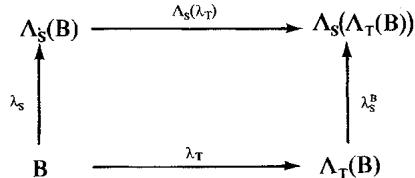
\includegraphics[keepaspectratio]{images/part001_09ec3539.jpg}}

is commutative. It suffices to check it on a generating set of the ring B.)

\begin{enumerate}
\def\labelenumi{\alph{enumi})}
\setcounter{enumi}{1}
\tightlist
\item
  Let C be a \(\lambda\)-ring, \(\rho:A \to C\) a \(\lambda\)-morphism, and \((c_i)_{i\in I}\) a family of elements of C. There exists one and only one \(\lambda\)-morphism \(\rho':B \to C\) extending \(\rho\) and such that \(\rho'(X_i) = c_i\) for all \(i\in I\).
\end{enumerate}

\begin{enumerate}
\def\labelenumi{\arabic{enumi})}
\setcounter{enumi}{51}
\tightlist
\item
  Let \((\mathbf{A}_i)_{i\in I}\) be a family of rings, \(\mathbf{A} = \prod_i\mathbf{A}_i\), and \(p_i:\mathbf{A}\to \mathbf{A}_i\) the canonical projection for every \(i\in \mathbf{I}\).\\
\end{enumerate}

\begin{enumerate}
\def\labelenumi{\alph{enumi})}
\item
  The map \(\alpha :\mathbf{A}[[T]]\to \prod_i\mathbf{A}_i[[T]]\) which maps \(\sum a_n\mathbf{T}^n\) onto \((\sum_{n}p_i(a_n)\mathbf{T}^n)_{i\in I}\) is a ring isomorphism. It defines, by restriction, a ring isomorphism \(\alpha :\Lambda (\mathbf{A})\to \prod_i\Lambda (\mathbf{A}_i)\). Moreover, we have, for all \(n\in \mathbf{J}\), \(\alpha \circ \lambda_n^{\mathbf{A}} = (\prod_i\lambda_n^{\mathbf{A}_i})\circ \alpha\) (Use the “universal polynomials” of Exerc. 46, d), p.~59.)
\item
  Suppose that, for every \(i \in I\), \(A_i\) is equipped with a structure \(\lambda_i: A_i \to \Lambda(A_i)\) of pre-\(\lambda\)-ring. By identifying \(\Lambda(A)\) with \(\prod_{i} \Lambda(A_i)\) by means of \(\alpha\), we define \(\lambda = \prod_{i} \lambda_i: A \to \Lambda(A)\). Then \((A, \lambda)\) is a pre-\(\lambda\)-ring, called the product of the family \(((A_i, \lambda_i))_{i \in I}\). For \((A, \lambda)\) to be a \(\lambda\)-ring, it is necessary and sufficient that \((A_i, \lambda_i)\) be one for all \(i \in I\).
\end{enumerate}

\begin{enumerate}
\def\labelenumi{\arabic{enumi})}
\setcounter{enumi}{52}
\tightlist
\item
  Let \(u = 1 + \mathrm{T} + \sum_{n=2}^{\infty} a_n \mathrm{T}^n\) be an element of \(\Lambda(\mathbf{Z})\). There exists one and only one group homomorphism \(\lambda^u: \mathbf{Z} \to \Lambda(\mathbf{Z})\) such that \(\lambda^u(1) = u\), and \((\mathbf{Z}, \lambda^u)\) is a pre-\(\lambda\)-ring. We have \(\lambda^u(n) = u^n\) for all \(n \in \mathbf{Z}\). For \((\mathbf{Z}, \lambda^u)\) to be a \(\lambda\)-ring, it is necessary and sufficient that \(u = 1 + \mathrm{T}\), in which case we have
\end{enumerate}

\[
\lambda_ {m} ^ {1 + \mathrm{T}} (n) = \binom {n} {m} = \frac {n (n - 1) \dots (n - m + 1)}{m !}
\]

for any \(n \in Z\) and \(m \in N\) .

\begin{enumerate}
\def\labelenumi{\arabic{enumi})}
\setcounter{enumi}{53}
\tightlist
\item
  Let C be a ring and A a C-algebra (not necessarily commutative). We denote \(\mathrm{Rep}_{\mathrm{C}}(\mathbf{A})\) the additive set of classes of A-modules that are finitely generated projective C-modules, and we denote \(\bar{\mathrm{R}}_{\mathrm{C}}(\mathring{\mathrm{A}})\) the Grothendieck group K( \(\mathrm{Rep}_{\mathrm{C}}(\mathbf{A})\) ) (cf.~A, VIII, § 10, n° 6). a) Let \(\alpha : \mathrm{A}' \to \mathrm{A}\) be a homomorphism of C-algebras. If E is an A-module of type \(\mathrm{Rep}_{\mathrm{C}}(\mathbf{A})\), then the module \(\alpha_{*}\mathrm{E}\), obtained by restriction of scalars from A to \(\mathrm{A}'\) (A, II, p.~30), is an A'-module of type \(\mathrm{Rep}_{\mathrm{C}}(\mathrm{A}')\), and {[}E{]} \(\mapsto [\alpha_{*}\mathrm{E}]\) defines a homomorphism \(\alpha_{*}: \mathrm{R}_{\mathrm{C}}(\mathrm{A}) \to \mathrm{R}_{\mathrm{C}}(\mathrm{A}')\).
\end{enumerate}

If \(\alpha_{1}:\mathbf{A}_{1}\to\mathbf{A}^{\prime}\) is a homomorphism of C-algebras, we have \((\alpha\circ\alpha_{1})_{*}=\alpha_{1*}\circ\alpha_{*}\) .

\begin{enumerate}
\def\labelenumi{\alph{enumi})}
\setcounter{enumi}{1}
\item
  One sets \(\mathbf{K}_0(\mathbf{C}) = \mathbf{R}_{\mathbf{C}}(\mathbf{C})\) . The structural homomorphism \(\varepsilon: \mathbf{C} \to \mathbf{A}\) defines a homomorphism \(\varepsilon_*: \mathbf{R}_{\mathbf{C}}(\mathbf{A}) \to \mathbf{K}_0(\mathbf{C})\) . If there exists a homomorphism \(\gamma: \mathbf{A} \to \mathbf{C}\) of C-algebras, then \(\gamma_*: \mathbf{K}_0(\mathbf{C}) \to \mathbf{R}_{\mathbf{C}}(\mathbf{A})\) is a right inverse of \(\varepsilon_*\) .
\item
  Let \(\gamma: \mathrm{C} \to \mathrm{C}'\) be a ring homomorphism. If E is an A-module of type \(\operatorname{Rep}_{\mathrm{C}}(\mathrm{A})\), then \(\gamma^{*}\mathrm{E} = \mathrm{C}' \otimes_{\mathrm{C}} \mathrm{E}\) is an \(\mathrm{A}_{\mathrm{C}'}\)-module of type \(\operatorname{Rep}_{\mathrm{C}'}(\mathrm{A}_{\mathrm{C}'})\), where \(\mathrm{A}_{\mathrm{C}'} = \mathrm{C}' \otimes_{\mathrm{C}} \mathrm{A}\), and {[}E{]} \(\mapsto [\gamma^{*}\mathrm{E}]\) defines a homomorphism \(\gamma^{*}: \mathrm{R}_{\mathrm{C}}(\mathrm{A}) \to \mathrm{R}_{\mathrm{C}'}(\mathrm{A}_{\mathrm{C}'})\). If \(\gamma_{1}': \mathrm{C}' \to \mathrm{C}_{1}\) is another ring homomorphism, we have \((\gamma_{1} \circ \gamma)^{*} = \gamma_{1}^{*} \circ \gamma^{*}\).
\item
  Let E \(\xrightarrow{f}\) F \(\xrightarrow{g}\) G be homomorphisms of A-modules, and set \(h = g \circ f\) . Construct an exact sequence of A-modules
\end{enumerate}

\[
(*) \quad 0 \rightarrow \operatorname{Ker} (f) \rightarrow \operatorname{Ker} (h) \rightarrow \operatorname{Ker} (g) \rightarrow \operatorname{Coker} (f) \rightarrow \operatorname{Coker} (h) \rightarrow \operatorname{Coker} (g) \rightarrow 0.
\]

Deduce from this that if \(f\) and \(g\) are injective, and if \(\operatorname{Coker}(f)\) and \(\operatorname{Coker}(g)\) are of type \(\operatorname{Rep}_{\mathbb{C}}(\mathbf{A})\), then \(\operatorname{Coker}(h)\) is of type \(\operatorname{Rep}_{\mathbb{C}}(\mathbf{A})\), and we have

\[
[ \operatorname{Coker} (h) ] = [ \operatorname{Coker} (f) ] + [ \operatorname{Coker} (g) ]
\]

in \(R_{C}(A)\) .

\begin{enumerate}
\def\labelenumi{\arabic{enumi})}
\setcounter{enumi}{54}
\tightlist
\item
  Let C be a ring. Let G be a monoid and let \(\mathbf{C}^{(\mathbf{G})}\) be its algebra over C. Instead of \(\mathrm{Rep}_{\mathbf{C}}(\mathbf{C}^{(\mathbf{G})})\) and \(\mathbf{R}_{\mathbf{C}}(\mathbf{C}^{(\mathbf{G})})\) , we write \(\mathrm{Rep}_{\mathbf{C}}(\mathbf{G})\) and \(\mathbf{R}_{\mathbf{C}}(\mathbf{G})\) . If \(\alpha : \mathbf{G}' \to \mathbf{G}\) is a homomorphism of monoids, we also denote by \(\alpha\) the homomorphism of C-algebras \(\mathbf{C}^{(\mathbf{G}')} \to \mathbf{C}^{(\mathbf{G})}\) that it defines, and \(\alpha_{*}: \mathbf{R}_{\mathbf{C}}(\mathbf{G}) \to \mathbf{R}_{\mathbf{C}}(\mathbf{G}')\) the corresponding homomorphism.
\end{enumerate}

By A, VIII, § 10, no. 5, there exists on R \(_{C}\) (G) a (commutative) ring structure such that

\[
[ \mathbf {E} ]. [ \mathbf {F} ] = [ \mathbf {E} \otimes_ {\mathrm{C}} \mathbf {F} ]
\]

if E and F are modules of finite type \(\mathrm{Rep}_{\mathbb{C}}(\mathbf{G})\) . The identity element for this multiplication is the class of the module \(C_1\) , equal to C with trivial action of G.

\begin{enumerate}
\def\labelenumi{\alph{enumi})}
\tightlist
\item
  The ring \(\mathbf{R}_{\mathrm{C}}(\mathbf{G})\) admits a unique structure of pre- \(\lambda\) -ring such that
\end{enumerate}

\[
\lambda [ \mathrm{E} ] = \sum_ {n \geqslant 0} \left[ \Lambda ^ {n} (\mathrm{E}) \right] \mathbf {T} ^ {n}
\]

for every module E of finite type \(\mathrm{Rep}_{\mathrm{C}}(\mathrm{G})\) . (First observe that \(\Lambda^{\mathrm{n}}(\mathrm{E})\) is again a module of finite type \(\mathrm{Rep}_{\mathrm{C}}(\mathrm{G})\) . Then, if F is a submodule such that F and E/F are of finite type \(\mathrm{Rep}_{\mathrm{C}}(\mathrm{G})\) , show that

\[
\left[ \Lambda ^ {n} (\mathrm{E}) \right] = \sum_ {p = 0} ^ {n} \left[ \Lambda ^ {p} (\mathrm{F}) \otimes_ {\mathrm{C}} \Lambda ^ {n - p} (\mathrm{E/F}) \right].
\]

in \(\mathbf{R}_{\mathbf{C}}(\mathbf{G})\).) For this, denote by \(\mathbf{L}_p\) the image of \(\Lambda^p(\mathbf{F}) \otimes_{\mathbf{C}} \Lambda^{n-p}(\mathbf{E})\), under the multiplication, in \(\Lambda^n(\mathbf{E})\). We have \(\Lambda^n(\mathbf{E}) = \mathbf{L}_0 \supset \mathbf{L}_1 \supset \ldots \supset \mathbf{L}_n = \Lambda^n(\mathbf{F}) \supset \mathbf{L}_{n+1} = 0\), and there exists a canonical isomorphism of \(\mathbf{C}^{(\mathbf{G})}\)-modules from \(\mathbf{L}_p / \mathbf{L}_{p+1}\) onto \(\Lambda^p(\mathbf{F}) \otimes \Lambda^{n-p}(\mathbf{E}/\mathbf{F})\).

\begin{enumerate}
\def\labelenumi{\alph{enumi})}
\setcounter{enumi}{1}
\item
  For every homomorphism \(\alpha: \mathbf{G}' \to \mathbf{G}\) of monoids, the map \(\alpha_*: \mathbf{R}_{\mathbf{C}}(\mathbf{G}) \to \mathbf{R}_{\mathbf{C}}(\mathbf{G}')\) is a \(\lambda\)-morphism. In particular \(\mathbf{K}_0(\mathbf{C})\) is a pre-\(\lambda\)-ring and \(\varepsilon_*: \mathbf{R}_{\mathbf{C}}(\mathbf{G}) \to \mathbf{K}_0(\mathbf{C})\) is a \(\lambda\)-morphism. The homomorphism \(\mathbf{G} \to \{1\}\) provides a right inverse for it.
\item
  Let \(\mathbf{G}\) a monoid and \(\mathbf{R}\) a set. A function \(f: \mathbf{G} \to \mathbf{R}\) will be called central if \(f(st) = f(ts)\) for any \(s, t \in \mathbf{G}\) . Let FC(G, R) denote the set of these functions. If R is a \(\lambda\) -ring, FC(G, R) is canonically endowed with a structure of \(\lambda\) -ring such that
\end{enumerate}

\[
\begin{array}{r l} (f + f ^ {\prime}) (s) & = f (s) + f ^ {\prime} (s) \\ (f \cdot f ^ {\prime}) (s) & = f (s) \cdot f ^ {\prime} (s) \\ (\lambda_ {n} f) (s) & = \lambda_ {n} (f (s)) \end{array}
\]

for any \(f, f'\) in \(\mathrm{FC}(\mathbf{G}, \mathbf{R})\) and \(s\) in \(\mathbf{G}\) . This applies in particular when \(\mathbf{R} = \Lambda(\mathbf{C})\) .

\begin{enumerate}
\def\labelenumi{\alph{enumi})}
\setcounter{enumi}{3}
\tightlist
\item
  Let E be a module of finite type \(\mathrm{Rep}_{\mathbb{C}}(\mathbf{G})\) . For every \(s \in \mathbf{G}\) , denote by \(s_{\mathbb{E}}\) the homothety of ratio \(s\) in E, and set
\end{enumerate}

\[
\overline {{{{\chi}}}} _ {\mathrm{E}} (s) = \det _ {\mathrm{E} [ \mathrm{T} ]} (1 + s _ {\mathrm{E}} \mathrm{T}) \in \Lambda (\mathrm{C})
\]

(cf. p. 62, exerc. 49). Show that

\[
\overline {{{{\chi}}}}: [ \mathrm{E} ] \mapsto \overline {{{{\chi}}}} _ {\mathrm{E}}
\]

defines a λ-morphism

\[
\overline {{{{\chi}}}}: \mathrm{R} _ {\mathrm{C}} (\mathrm{G}) \rightarrow \mathrm{FC} (\mathrm{G}, \Lambda (\mathrm{C})).
\]

\begin{enumerate}
\def\labelenumi{\alph{enumi})}
\setcounter{enumi}{4}
\tightlist
\item
  If C is a field, then \(\overline{\chi}\) is injective (A, VIII, § 10, no. 6, prop. 10). Deduce in this case that \(R_{C}(G)\) is a \(\lambda\)-ring.
\end{enumerate}

\begin{enumerate}
\def\labelenumi{\arabic{enumi})}
\setcounter{enumi}{55}
\tightlist
\item
  Let G be the free monoid generated by an element T, so that \(\mathrm{C}^{(\mathrm{G})}\) is identified with C{[}T{]}. Denote by \(C_{0}\) the module \(C{[}T{]}/T C{[}T{]}\). Then \([C_{0}]\) is an idempotent element of \(\mathrm{R}_{\mathrm{C}}(\mathrm{C}[\mathrm{T}])\). The kernel of the canonical \(\lambda\)-morphism \(\mathrm{R}_{\mathrm{C}}(\mathrm{C}[\mathrm{T}]) \rightarrow \mathrm{K}_{0}(\mathrm{C})\) is the ideal generated by \(1 - [\mathrm{C}_{0}]\). Put
\end{enumerate}

\[
\tilde {\mathrm{R}} _ {\mathrm{C}} (\mathrm{C} [ \mathrm{T} ]) = \mathrm{R} _ {\mathrm{C}} (\mathrm{C} [ \mathrm{T} ]) / [ \mathrm{C} _ {0} ]. \mathrm{R} _ {\mathrm{C}} (\mathrm{C} [ \mathrm{T} ]).
\]

\begin{enumerate}
\def\labelenumi{\alph{enumi})}
\item
  Show that \([C_{0}].R_{C}(C[T])\) is a \(\lambda\)-ideal, hence that \(\tilde{R}_{C}(C[T])\) admits a quotient pre-\(\lambda\)-ring.
\item
  For every module E of finite type \(\operatorname{Rep}_{\mathbf{C}}(\mathbf{C}[\mathbf{T}])\) , denote by \(\mathbf{T}_{\mathbf{E}}\) the homothety of ratio T in E. We have
\end{enumerate}

and

\[
\begin{array}{l} \overline {{\chi}} _ {\mathrm{E}} (\mathrm{T}) = \det _ {\mathrm{E} [ \mathrm{T} ]} (1 + \mathrm{T} _ {\mathrm{E}} \mathrm{T}) \in \Lambda (\mathrm{C}) \\ \chi_ {\mathrm{E}} (\mathrm{T}) = \det _ {\mathrm{E} [ \mathrm{T} ]} (\mathrm{T} - \mathrm{T} _ {\mathrm{E}}) \end{array}
\]

is the characteristic polynomial of \(T_{E}\) (cf.~exerc. 49, p.~62). Show that \([E] \mapsto \overline{\chi}_{E}(T)\) defines a \(\lambda\) -morphism \(R_{C}(C[T]) \to \Lambda(C)\) whose kernel contains \([C_{0}]\) . By passing to the quotient, we obtain a \(\lambda\) -morphism

\[
\overline {{\chi}}: \tilde {\mathrm{R}} _ {\mathrm{C}} (\mathrm{C} [ \mathrm{T} ]) \to \Lambda (\mathrm{C}).
\]

\begin{enumerate}
\def\labelenumi{\alph{enumi})}
\setcounter{enumi}{2}
\item
  Denote by \(\Lambda_{\mathrm{rat}}(\mathbf{C})\) the subgroup of \(\Lambda(\mathbf{C})\) generated by the elements of \(\Lambda(\mathbf{C})\) which are polynomials in T. Show that the image of \(\overline{\chi}\) is \(\Lambda_{\mathrm{rat}}(\mathbf{C})\). Conclude from this that \(\Lambda_{\mathrm{rat}}(\mathbf{C})\) is a sub-\(\lambda\)-ring of \(\Lambda(\mathbf{C})\).
\item
  For every \(r \in \mathbf{Z}\), define \(\sigma_r: \mathrm{C}[\mathrm{T}, \mathrm{T}^{-1}] \to \mathrm{C}[\mathrm{T}, \mathrm{T}^{-1}]\) by \((\sigma_r f)(\mathrm{T}) = \mathrm{T}^{r} f((-\mathrm{T})^{-1})\). We have \((\sigma_r(\sigma_s f))(\mathrm{T}) = (-1)^s \mathrm{T}^{r-s} f(\mathrm{T})\), in particular \(\sigma_r(\sigma_r f) = (-1)^r f\), and \((\sigma_r f).(\sigma_s g) = \sigma_{r+s}(f.g)\), for all \(r, s\) in \(\mathbf{Z}\) and \(f, g\) in \(\mathrm{C}[\mathrm{T}, \mathrm{T}^{-1}]\). If \(f\) is a polynomial in \(T\) of degree \(\leqslant r\) (\(r \geqslant 0\)), then \(\sigma_r f\) is one as well. If moreover \(f \in \Lambda(\mathrm{C})\) (i.e. \(f(0) = 1\)), then \(\sigma_r f\) is monic of degree \(r\). If E is a C{[}T{]}-module which is a free C-module of rank \(r\), one has \(\sigma_r(\overline{\chi}_{\mathrm{E}}(\mathrm{T})) = \chi_{\mathrm{E}}(\mathrm{T})\). e) If \(f \in \Lambda(\mathrm{C})\) is a polynomial in \(T\) of degree \(\leqslant r\), set \(E_{r,f} = C[T]/\sigma_r f.C[T]\); it is a free C-module of rank \(r\). If \(f = 1\) we have \(E_{r,1} = C[T]/T^{r}C[T]\). If \(g \in \Lambda(\mathrm{C})\) is a polynomial in \(T\) of degree \(\leqslant s\), we have an exact sequence of C{[}T{]}-modules
\end{enumerate}

\[
(*) \quad 0 \rightarrow \mathrm{E} _ {s, g} \rightarrow \mathrm{E} _ {r + s, f g} \rightarrow \mathrm{E} _ {r, f} \rightarrow 0
\]

(using \(d\) ). Show that the class \(\tau(f)\) of \(\mathrm{E}_{r,f}\) in \(\tilde{\mathrm{R}}_{\mathrm{C}}(\mathrm{C}[\mathrm{T}])\) is independent of \(r\) ( \(\geqslant \deg(f)\) ). (Indeed \(\sigma_{r+s}f = (\sigma_s1).(\sigma_rf) = \mathrm{T}^s.(\sigma_rf)\) and the class of the module \(\mathrm{C}[\mathrm{T}] / \mathrm{T}^s\mathrm{C}[\mathrm{T}]\) in \(\tilde{\mathrm{R}}_{\mathrm{C}}(\mathrm{C}[\mathrm{T}])\) is zero.) Show that if \(g\) is a polynomial in \(\Lambda(\mathrm{C})\) , one has \(\tau(fg) = \tau(f) + \tau(g)\) . (Use again the exact sequence (*).) Deduce from this that \(\tau\) extends to a group homomorphism

\[
\tau : \Lambda_ {\mathrm{rat}} (\mathrm{C}) \rightarrow \tilde {\mathrm{R}} _ {\mathrm{C}} (\mathrm{C} [ \mathrm{T} ]).
\]

\begin{enumerate}
\def\labelenumi{\alph{enumi})}
\setcounter{enumi}{5}
\tightlist
\item
  Show that \(\overline{\chi} \circ \tau\) is the identity map of \(\Lambda_{\mathrm{rat}}(\mathbf{C})\) (Using the fact that if \(f \in \Lambda(\mathbf{C})\) is a polynomial of degree \(\leqslant r\), then the characteristic polynomial of \(\mathrm{T}_{\mathrm{E}_r,f}\) is \(\sigma_r f\).)
\item
  Show that every element of \(\tilde{\mathrm{R}}_{\mathrm{C}}(\mathrm{C}[\mathrm{T}])\) is the class of a C{[}T{]}-module E which is a free C-module.
\end{enumerate}

\(h\) ) Let E be a C{[}T{]}-module, and denote by \(u\in \mathrm{End}_{\mathrm{C}}(\mathrm{E})\) the homothety of ratio T in E; let \(\overline{u} = \mathrm{Id}_{\mathrm{C[T]}}\otimes_{\mathrm{C}}u\in \mathrm{End}_{\mathrm{C[T]}}(\mathrm{E}[\mathrm{T}])\). We have an exact sequence of C{[}T{]}-modules

\[
0 \longrightarrow \mathrm{E} [ \mathrm{T} ] \xrightarrow {\mathrm{T} - \bar {u}} \mathrm{E} [ \mathrm{T} ] \longrightarrow \mathrm{E} \longrightarrow 0
\]

(A, III, p.~106). Suppose that E is a free C-module with basis \((e_1, \ldots, e_r)\). Then E{[}T{]} is a free C{[}T{]}-module with basis \((1 \otimes e_i)\). If the matrix of \(u\) for the basis \((e_i)\) is \((a_{ij})\), the matrix of T - \(\overline{u}\) for the basis \((1 \otimes e_i)\) is \((\mathrm{T}\delta_{ij} - a_{ij})\).

\begin{enumerate}
\def\labelenumi{\roman{enumi})}
\tightlist
\item
  Let \(f = (f_{ij})_{1 \leqslant i,j \leqslant r}\) be a matrix with coefficients in C{[}T{]}. We say that \(f\) is special if, for all \(i, j\) in \(\{1, \dots, r\}\), \(i \neq j\), \(f_{ii}\) is a monic polynomial and \(\deg(f_{ii}) > \deg(f_{ij})\). Then show that \(\det(f)\) is a monic polynomial (of degree \(\deg(f_{11}) + \cdots + \deg(f_{rr})\)) and that \(f\) defines an injective endomorphism of C{[}T{]} \(^r\). Deduce from h) that every C{[}T{]}-module which is a free C-module of rank \(r\) is isomorphic to the cokernel of such an endomorphism of C{[}T{]} \(^r\).
\end{enumerate}

\begin{enumerate}
\def\labelenumi{\alph{enumi})}
\setcounter{enumi}{9}
\tightlist
\item
  Let f be a special matrix as in i). Set \(f = \begin{pmatrix} f_{11} & f_{+} \\ f_{-} & f' \end{pmatrix}\) where \(f_{+}\) , \(f_{-}\) , \(f'\) are matrices of types \((1, r - 1)\) , \((r - 1, 1)\) and \((r - 1, r - 1)\) respectively. Set
\end{enumerate}

\[
g = \left( \begin{array}{c c} 1 & 0 \\ - f _ {-} & f _ {1 1} \mathrm{I} \end{array} \right) \quad \text {and} \quad h = g f = \left( \begin{array}{c c} f _ {1 1} & f _ {+} \\ 0 & \overline {{f}} \end{array} \right) \quad \text {where} \quad \overline {{f}} = f _ {1 1} f ^ {\prime} - f _ {-} f _ {+}.
\]

Show that h is a special matrix. Moreover, by identifying square matrices with the corresponding endomorphisms, one obtains exact sequences of C{[}T{]}-modules

\[
0 \rightarrow \operatorname{Coker} (f) \rightarrow \operatorname{Coker} (h) \rightarrow \operatorname{Coker} (g) \rightarrow 0,
\]

(where Coker(g) is isomorphic to \(\mathbf{C}[\mathbf{T}]^{r - 1} / f_{11}\mathbf{C}[\mathbf{T}]^{r - 1}\) ) and

\[
0 \rightarrow \mathrm{C} [ \mathrm{T} ] / f _ {1 1} \mathrm{C} [ \mathrm{T} ] \rightarrow \operatorname{Coker} (h) \rightarrow \operatorname{Coker} (\bar {f}) \rightarrow 0.
\]

From this, deduce by induction on \(r\) that \(\operatorname{Coker}(f)\) is a projective C-module whose class in \(\mathbf{R}_{\mathrm{C}}(\mathbf{C}[\mathrm{T}])\) is a \(\mathbf{Z}\)-linear combination of elements of the form \([\mathbf{C}[\mathrm{T}] / p\mathbf{C}[\mathrm{T}]]\), where \(p\) is a monic polynomial.

  \(k\) ) Use parts \(f\), \(g\), \(i)\), and \(j)\) above to show that \(\tau : \Lambda_{\mathrm{rat}}(\mathbf{C}) \to \tilde{\mathbf{R}}_{\mathrm{C}}(\mathbf{C}[\mathrm{T}])\) is surjective, hence that \(\overline{\chi} : \tilde{\mathbf{R}}_{\mathrm{C}}(\mathbf{C}[\mathrm{T}]) \to \Lambda_{\mathrm{rat}}(\mathbf{C})\) is an isomorphism.

\begin{enumerate}
\def\labelenumi{\alph{enumi})}
\setcounter{enumi}{11}
\tightlist
\item
  Show that \(\Lambda_{\mathrm{rat}}(\mathbf{C})\) is stable under \(\mathbf{V}_n\) and \(\mathbf{F}_n\) for each \(n \in \mathbf{J}\). There therefore correspond to them endomorphisms \(\mathbf{V}_n\) and \(\mathbf{F}_n\) of \(\tilde{\mathbf{R}}_{\mathbf{C}}(\mathbf{C}[\mathbf{T}])\), by the preceding isomorphism. Let \(\varphi_n\) be the homomorphism of C-algebras from C{[}T{]} to itself which maps T to \(\mathbf{T}^n\). Show that \(\mathbf{V}_n\) (resp. \(\mathbf{F}_n\)) is deduced from the endomorphism \(\varphi_n^*\) (resp. \((\varphi_n)_*\)) of \(\mathbf{R}_{\mathbf{C}}(\mathbf{C}[\mathbf{T}])\) by passing to quotients.
\end{enumerate}

In the following exercises, p is a fixed prime number, and the rings of Witt vectors are relative to this prime number.

\begin{enumerate}
\def\labelenumi{\arabic{enumi})}
\setcounter{enumi}{56}
\tightlist
\item
  Let \(m\), \(n\) be two integers \(\geqslant 1\). For every ring A of characteristic \(p\), denote by \(_{m}\mathrm{W}_{n}(\mathrm{A})\) the kernel of the endomorphism \(\mathrm{F}^{m}\) of \(\mathrm{W}_{n}(\mathrm{A})\).
\end{enumerate}

\begin{enumerate}
\def\labelenumi{\alph{enumi})}
\tightlist
\item
  For \(m \geqslant 2\) and \(n \geqslant 1\) the following diagram is commutative
\end{enumerate}

\pandocbounded{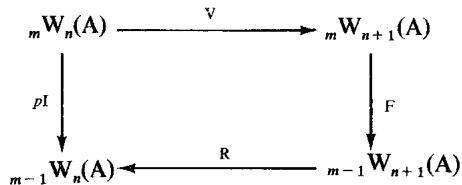
\includegraphics[keepaspectratio]{images/part001_6a9997c3.jpg}}

where the maps V, F are induced by the shift and Frobenius homomorphisms, respectively, I is the natural injection, and R is the natural projection.

\begin{enumerate}
\def\labelenumi{\alph{enumi})}
\setcounter{enumi}{1}
\tightlist
\item
  For \(n \geqslant 1\) and \(a = [a_0, \ldots, a_{n-1}]\) in \(W_n(A)\) , denote by \(\tilde{a}\) the element \((a_0, \ldots, a_{n-1}, 0, \ldots)\) of \(W(A)\) .
\end{enumerate}

Let \(a \in_{m} W_{n}(A)\) , \(b \in_{n} W_{m}(A)\) We then set

\[
\langle \boldsymbol {a}, \boldsymbol {b} \rangle = \mathrm{E} (\omega_ {\mathrm{A}} (\tilde {\boldsymbol {a}}) \omega_ {\mathrm{A}} (\tilde {\boldsymbol {b}}), 1)
\]

(cf. p. 57, exerc. 43 for the notation E, and p. 54, exerc. 40 for the notation \(\omega_{\mathbf{A}}\) ). Prove that the map \((\boldsymbol{a}, \boldsymbol{b}) \mapsto \langle \boldsymbol{a}, \boldsymbol{b} \rangle\) from \({}_{m}W_n(A) \times {}_{n}W_m(A)\) into \(A^*\) is \(\mathbf{Z}\)-bilinear. c) With the notation of a), we have

\[
\langle \boldsymbol {a}, \mathrm{V} \boldsymbol {b} \rangle = \langle \mathrm{F} \boldsymbol {a}, \boldsymbol {b} \rangle . \text { for } \quad \boldsymbol {a} \in_ {m} \mathrm{W} _ {n} (\mathrm{A}) \quad \text { and } \quad \boldsymbol {b} \in_ {n} \mathrm{W} _ {m - 1} (\mathrm{A})
\]

and

\[
\langle \mathbf {R} \boldsymbol {a}, \boldsymbol {b} \rangle = \langle \boldsymbol {a}, \mathbf {I} \boldsymbol {b} \rangle \quad \text { for } \quad \boldsymbol {a} \in_ {m} \mathrm{W} _ {n} (\mathrm{A}) \quad \text { and } \quad \boldsymbol {b} \in_ {n - 1} \mathrm{W} _ {m} (\mathrm{A}).
\]

\begin{enumerate}
\def\labelenumi{\arabic{enumi})}
\setcounter{enumi}{57}
\tightlist
\item
  \begin{enumerate}
  \def\labelenumii{\alph{enumii})}
  \tightlist
  \item
    Let \(\delta(T)\) be the formal series \(\exp\left(-\sum_{n=0}^{\infty}\mathrm{T}^{p^n}/p^n\right)\) of \(\mathbf{Q}[[T]]\). We have
  \end{enumerate}
\end{enumerate}

\[
\mathfrak{E}(\mathrm{T}) = \prod_{\substack{(n,p) = 1\\ n\text{ an integer}\geqslant 1}}(1 - \mathrm{T}^{n})^{\mu (n) / n}
\]

where μ is the Möbius function. The coefficients of δ(T) belong to \(\mathbf{Z}_{(p)}\). b) Let \(\mathbf{X} = (\mathbf{X}_{n})_{n \in \mathbb{N}}\) be a family of indeterminates. In the algebra \(\mathbf{Q}[(\mathbf{X}_{n})_{n \in \mathbb{N}}]\), we have the equality

\[
\prod_ {n = 0} ^ {\infty} \mathcal {E} (\mathrm{X} _ {n} \mathrm{T} ^ {p ^ {n}}) = \exp \left(- \sum_ {n = 0} ^ {\infty} \Phi_ {n} (\mathrm{X}) \mathrm{T} ^ {p ^ {n}} / p ^ {n}\right).
\]

\begin{enumerate}
\def\labelenumi{\alph{enumi})}
\setcounter{enumi}{2}
\item
  Let A be a \(\mathbf{Z}_{(p)}\) -algebra. It is assumed that multiplication by \(p, 1_{\mathbf{A}}\) is injective in A. Let \(\boldsymbol{a} = (a_n)_{n \in \mathbb{N}} \in \mathbb{A}^{\mathbf{N}}\) . For the series \(\exp\left(\sum_{n=0}^{\infty} a_n \mathbf{T}^{p^n} / p^n\right)\) of \(\mathrm{A}\left[\frac{1}{p}\right]\) {[}{[}T{]}{]} to have its coefficients in A, it is necessary and sufficient that \(\boldsymbol{a}\) belongs to \(\Phi_{\Lambda}(\mathbf{W}(\mathbf{A}))\) .
\item
  Let A be a \(\mathbf{Z}_{(p)}\)-algebra. The map \(\mathbf{E} \circ \omega_{\Lambda}\) from W(A) to \(\Lambda(\mathbf{A})\) (cf.~p.~54, exerc. 40 and p.~57, exerc. 43) associates to \(\boldsymbol{a} = (a_n)_{n \in \mathbb{N}}\) the element \(\prod_{n=0}^{\infty} \delta(a_n(-\mathbf{T})^{p^n})\) of \(\Lambda(\mathbf{A})\).
\item
  Let A be a \(\mathbf{Z}_{(p)}\)-algebra. Suppose that multiplication by \(p,1_{A}\) is injective in A. Let \(\sigma\) be an endomorphism of A satisfying \(\sigma a \equiv a^{p} \mod pA\). Let \(s_{\sigma}:A \to W(A)\) be the homomorphism associated with \(\sigma\) (p.~44, exerc. 14). Then, for every \(a \in A\), the formal series
\end{enumerate}

\[
\mathrm{E} _ {\sigma} (a, \mathrm{T}) = \exp (\sum_ {i = 0} ^ {\infty} \sigma^ {i} (a) \mathrm{T} ^ {p ^ {i}} / p ^ {i})
\]

has its coefficients in A, and we have

\[
\mathrm{E} \circ \omega_ {\mathrm{A}} \circ s _ {\sigma} (a ^ {- 1}) = \exp \left(\sum_ {i = 0} ^ {\infty} \sigma^ {i} (a) (- \mathrm{T}) ^ {p ^ {i}} / p ^ {i}\right) = \mathrm{E} _ {\sigma} (a, - \mathrm{T}).
\]

\begin{enumerate}
\def\labelenumi{\alph{enumi})}
\setcounter{enumi}{5}
\tightlist
\item
  Let \(\mathcal{A}\) the ring \(\mathbf{Z}_{(p)}[(\mathbf{X}_n)_{n\in\mathbb{N}}]\) and let \(\mathbf{X} = (\mathbf{X}_n)_{n\in\mathbb{N}} \in \mathrm{W}(\mathcal{A})\) . The series \(\mathrm{E}_{\mathrm{F},\mathcal{A}}(\mathbf{X},\mathrm{T})\) has its coefficients in \(\mathrm{W}(\mathcal{A})\) . For every \(\mathbf{Z}_{(p)}\) -algebra A and every element \(a = (a_n)_{n\in\mathbb{N}}\) of \(\mathrm{W}(\mathrm{A})\) , we shall write \(\mathrm{E}_{\mathrm{F}}(a,\mathrm{T})\) the series obtained by applying \(\mathrm{W}(\varphi)\) to the coefficients of \(\mathrm{E}_{\mathrm{F},\mathcal{A}}(\mathbf{X},\mathrm{T})\) where \(\varphi: \mathcal{A} \to \mathrm{A}\) is the map which to \(\mathrm{X}_n\) to \(a_n\) . Then \(\mathrm{E}_{\mathrm{F}}(a,\mathrm{T})\) has its coefficients in \(\mathrm{W}(\mathrm{A})\) and if \(s_{\mathrm{A}}\) denotes the homomorphism \(\mathrm{W}(\mathrm{A}) \to \mathrm{W}(\mathrm{W}(\mathrm{A}))\) defined in Exerc. 15, p.~44, we have
\end{enumerate}

\[
\mathrm{E} \circ \omega_ {\mathrm{W(A)}} \circ s _ {\mathrm{A}} (\boldsymbol {a} ^ {- 1}) = \mathrm{E} _ {\mathrm{F}} (\boldsymbol {a}, - \mathrm{T}) \quad \text { for all } \quad \boldsymbol {a} \in \mathrm{W(A)}.
\]

